\documentclass[a4paper,11pt,titlepage]{article}
\usepackage[T1]{fontenc}
\usepackage[utf8x]{inputenc}
\usepackage{polski}
%\usepackage[polish]{babel}
\usepackage{graphicx}
\usepackage{subfig}
\usepackage{placeins}
\usepackage{amsthm}
\newtheorem{hyp}{Hipoteza}[subsection]

\begin{document}
\title{Informatyku! Jak Ci się pracuje? \\ \Large Satysfakcją z~pracy oraz zaangażowanie w~pracę \\ wśród pracowników sektora IT.}
\author{\Large{Agnieszka Lewandowska} \\ \texttt{agnieszka.lewandowska@gmail.com} }
\date{czerwiec 2011}
\maketitle

%\begin{abstract}
%TODO napisz abstrakt :-)
%end{abstract}

\tableofcontents
\cleardoublepage

\section{Wstęp}
Zarządzanie zespołem nie jest trywialnym zadaniem. W ramach pracy z zespołem należy dopilnować poprawnego wykonania zadania, a także zarządzać ludźmi. Nie oznacza to tylko wyznaczania im zadań i pilnowania, aby wykonali je w założonym terminie. Zarządzanie zespołem ludzi to nie tyko zarządzanie zadaniami, ale także realizacja potrzeb pracowników.

Na skuteczność pracowników wpływa także stan psychiczny członków zespołu, nie tylko ich umiejętności. Za skutecznością idzie poprawność i skuteczność zleconych zadań, Dlatego też tak istotne jest rozeznanie w sprawie przyczyn danego działania pracowników -- zarówno czynów odbieranych negatywnie (wyeliminowanie) jak i wyjątkowo pozytywnie (podtrzymanie). Tą drugą częścią będzie zajmować się niniejsza praca -- przyczynami powodującymi dobre wykonywanie zadań, w określonych terminach, na
oczekiwanym poziomie (efekt zaangażowania w pracę). Ponadto będą badane przyczyny, które powodują, że pracownik chce w danej firmie zostać, jego podejście buduje dobrą atmosferę w pracy oraz pozytywnie wpływa na innych współpracowników (poziom satysfakcji z pracy). 

Należy pamiętać, że pracownicy niezadowoleni, jasno dający wyraz swojej frustracji, mogą zepsuć atmosferę w pracy i przelać swoje niezadowolenie na innych. Dodatkowo nieusatysfakcjonowany pracownik ma większą motywację do odejścia, co może być szkodliwe dla firmy, szczególnie gdy taka osoba ma odpowiednie doświadczenie, wiedzę oraz umiejętności. Jest zaufanym, sprawdzonym pracownikiem. Znalezienie osoby na zastępstwo zabiera czas, wyszkolenie i zbadanie jego
potencjalnych umiejętności, dodatkowo wydłużają proces podczas którego staje się przydatnym pracownikiem firmy.

Podsumowując, niniejsza praca ma za zadanie sprawdzić jak w Polsce, a dokładniej w Poznaniu, dba się o pracowników sektora IT. W szczególności badana jest satysfakcja z pracy oraz zaangażowanie w wykonywane zadania. Czy badana grupa zawodowa różni się od średniej Polaków,a może nie? Jaka jest charakterystyka tej grup i jak wiąże się z teorią odnośnie zaangażowania w pracę i satysfakcji z pracy?

\section{Satysfakcja z pracy i jej wymiary}
Zanim przejdziemy do pełnej definicji satysfakcji z pracy warto jasno określić czym jest satysfakcja. Wg Słownika języka polskiego PWN \citep{web:pwn-sat}
\begin{quote}
satysfakcja -- uczucie przyjemności i zadowolenia z czegoś
\end{quote}
Idąc tym tropem można przekształcić powyższą definicję na potrzeby tej pracy
\begin{quote}
satysfakcja z pracy -- uczucie przyjemności i zadowolenia z pracy
\end{quote}

Natomiast pełna definicja wg podręcznika psychologii \citep{SchultzSat} jest bardziej złożona i definiuje satysfakcje z pracy jako wielowymiarowy konstrukt, którego elementy składowe wciąż są odkrywane.

\begin{quotation}
Satysfakcję z pracy stanowią pozytywne i negatywne uczucia oraz postawy wobec naszej pracy. Zależy ona od wielu czynników związanych z pracą, poczynając od miejsca parkowania samochodu do poczucia samospełnienia przy realizacji codziennych zadań. Na satysfakcję z pracy mogą również wpływać czynniki indywidualne. Należą do nich wiek, stan zdrowia, staż pracy, stabilność emocjonalna, status społeczny, ulubione rozrywki czy też posiadanie rodziny i kontaktów społecznych. Nasza motywacja i
aspiracje, oraz sposób ich zaspokajania przez pracę, także wpływają na postawy wobec pracy.
\end{quotation}
Wśród innych, niewymienionych czynników wpływających na satysfakcję, wyróżnia się także:
\begin{itemize}
\item styl zarządzania,
\item kulturę w organizacji,
\item autonomię pracy,
\item nagrody i kary,
\item godziny pracy,
\item organizację pracy.
\end{itemize}
Czynniki te mogą być zależne od kraju i jego kultury, jak i od typu organizacji, czy typu wykonywanej pracy, a także zajmowanego stanowiska. Dla przykładu, dla pracownika przy taśmie autonomia w pracy będzie nieistotna, w przeciwieństwie do kadry kierowniczej, dla której to swoboda działania może być istotnym czynnikiem wpływającym na ich wydajność. Idąc dalej, dla pracownika w Stanach Zjednoczonych, gdzie nie ma darmowej służby zdrowia, dodatki, takie jak ubezpieczenie zdrowotne, są bardziej istotne niż w Polsce, gdzie prawo do opieki zdrowotnej wpisane jest w konstytucję. 

Należy tutaj podkreślić, że satysfakcja z pracy nie jest tym samym co motywacja do pracy, czy zaangażowanie w pracę. Intuicyjnie jednak, definicje te są ze sobą powiązane.

\subsection{Modele}
\subsubsection{Teoria wpływu -- Edwin A. Locke (1976)}

Teoria \citep{locke1976nature} opiera się na różnicy między oczekiwaniami pracownika, a rzeczywistością zastaną w pracy. Satysfakcja z pracy jest odwrotnie proporcjonalna do wielkości tej różnicy. Dla przykładu, optymalna godzina przybycia do pracy dla Anny to 9 rano. Natomiast pracodawca wymusza przybycie o 7 rano. Zgodnie z tą teorią zmniejsza to poziom satysfakcji z pracy u Anny. Z drugiej strony, jeżeli Annie by pozwolono na przychodzenie o 9 wpłynęłoby to na zwiększenie jej zadowolenia.

Dodatkowo teoria ta rozróżnia wagi pomiędzy różnymi wymiarami satysfakcji z pracy, tzn. każdy wymiar posiada inny, zależny od indywidualnych cech pracownika wpływ na zadowolenie. Obrazując to na wcześniej podanym przykładzie, w przeciwieństwie do Anny, dla Tomka godzina przyjścia do pracy ma minimalne znaczenie i w niewielkim stopniu wpływa na jego satysfakcję. Natomiast duże znaczenie dla niego ma werbalne docenienie ze strony kierownictwa. Z czego
wynika, że ze względu na poziom satysfakcji z pracy, Anna potrzebuje kierownika akceptującego elastyczne godziny pracy, natomiast Tomek -- osobę doceniającą jawnie dokonania swoich podwładnych.

Teoria wpływu jest to obecnie najbardziej znany model satysfakcji z pracy.

\subsubsection{Teoria dyspozycyjności -- Timothy A. Judge (1998)}
Teoria ta wychodzi z ogólnego założenie, że każdy człowiek ma swoje własne, wewnętrzne predyspozycje, które definiują u niego pewien określony poziom satysfakcji z pracy, niezależnie od wykonywanego zawodu czy zajmowanego stanowiska. Dla takich osób zewnętrzne czynniki, takie jak organizacja pracy, styl zarządzania czy inne, nie mają wpływu na satysfakcję.

Teoria ta jest zgodna z wynikami badań, że poziom zadowolenia z pracy ma tendencje do utrzymywania się na stałym poziomie w czasie oraz między stanowiskami, a także firmami w wypadku wybranych osób. Przykładem takich badań, są badania nad bliźniakami jednojajowymi, które wskazują właśnie na wpływ genów na poziomie 30-40\%  na zadowolenia z pracy. Jednak teoria ta jest krytykowana i istnieją już wyniki badań wskazujące na brak zależności \citep{schultz1985family}.

Szczególnym zawężeniem tej teorii, jest teoria \emph{Core Self-evaluations Model} zaproponowana przez Timothy A. Judge w 1998 \citep{judge1998dispositional,judge2001relationship}. Wg niej istnieją 4 podstawowe elementy samooceny związane z satysfakcją z pracy:
\begin{itemize}
\item poczucie własnej wartości -- wprost proporcjonalne,
\item ocena własnych umiejętności -- wprost proporcjonalne,
\item umiejscowienie kontroli -- wprost proporcjonalne do wewnętrznego poczucia kontroli (my wpływamy na sytuacje),
\item neurotyczność -- odwrotnie proporcjonalne.
\end{itemize}

\subsubsection{Teoria dwuczynnikowa (teoria motywacji-higieny) -- Fredereick Herzberg (1974)}
Teoria ta wskazuje dwa czynniki, które osobno wpływają na satysfakcje i brak satysfakcji; odpowiednio: motywacja oraz czynniki higieny \citep{herzberg1974motivation}. 

\paragraph{Motywacja.} Wyższa motywacja powoduje wzrost zadowolenia z pracy. Może być widziana jako czynniki wewnętrzne pchające pracownika do osiągnięcia prywatnych i organizacyjnych celów. Motywatorami są takie elementy pracy, które powodują chęć do działania i zapewniają uczucie zadowolenia w pracy:
\begin{itemize}
\item osiągnięcia w pracy, np.: zdobycie kolejnego klienta, zakończenie projektu sukcesem,
\item docenienie, np.: bonus za wydajność, pochwała na zebraniu pracowników,
\item możliwości promocji, np.: awans po roku pracy, szkolenia na wyższe stanowiska.
\end{itemize}
Motywatory te muszą być związane z wykonywaną pracą.

\paragraph{Higiena.} Natomiast czynniki higieny to czynniki związane ze środowiskiem pracy, takie jak:
\begin{itemize}
\item płaca -- wysokość wynagrodzenie w stosunku do włożonego wysiłku i wykonywanych zadań, 
\item nadzór -- kompetencje merytoryczne i sposób zarządzania,
\item organizacja w firmie -- sposób organizacji pracy ułatwiający wykonywanie zadań, 
\item niezależność -- możliwość wykonywania zadań w wybranych przez pracownika sposób,
\item docenienie -- pochwały za dobrze wykonaną pracę,
\item możliwość wykorzystania swoich zdolności,
\item moralność -- praca zgodna z wartościami moralnymi pracownika,
\item nagrody -- niezwiązane z pensją formy uznania: finansowe i pozafinansowe.
\end{itemize}

Teoria ta wzbudza kontrowersje, ze względu na nie branie pod uwagę cech indywidualnych pracowników, a co za tym idzie, te same reakcje na zmiany w motywatorach i czynnikach higieny przez każdego z pracowników. W teorii tej brakuje także wskazanej metody badania obu czynników, co powoduje, że jest ciężka do potwierdzenia empirycznie.

\subsubsection{Model charakterystyki pracy -- Hackam \& Oldham (1976)}
Teoria ta \citep{hackman1976motivation} wskazuje na pięć głównych cech pracy:
\begin{itemize}
\item różnorodność wymaganych umiejętności,
\item identyfikacja z zadaniem (dopasowanie zadań),
\item znaczenie zadania,
\item autonomia,
\item informacja zwrotna,
\end{itemize}
które wpływają na trzy stany emocjonalne
\begin{itemize}
\item poczucie sensowności,
\item odpowiedzialność,
\item znajomość wyników pracy,
\end{itemize}
które z kolei wpływają na efekty pracy, w tym na satysfakcję z pracy. 

Ze względu na szerszy charakter tej teorii, wykorzystywana jest ona do badania charakterystyki pracy (zawierającej poza zadowoleniem z pracy, takie elementy jak absencja czy motywacja do pracy), a nie tylko satysfakcji.

\subsection{Sposoby pomiaru}
Satysfakcja z pracy mierzona jest zazwyczaj przy pomocy kwestionariuszy, które badają ogólny poziom zadowolenia lub wybrane aspekty pracy związane z satysfakcją. Ankiety takie są rozsyłane lub rozdawane pracownikom, którzy są proszeni o anonimowe jej uzupełnienie. Dodatkowo badania są zazwyczaj dobrowolne. Powoduje to, że testy wypełniane są przez podzbiór wszystkich pracowników o nieznanej charakterystyce, np.: tylko najbardziej zaangażowani wypełniają testy. W
związku z tym ciężko stwierdzić jak zebrane wyniki odzwierciedlają rzeczywisty poziom zadowolenia wśród całej populacji badanych.

Przykładowym kwestionariuszem satysfakcji z pracy jest Minesocki Kwestionariusz Satysfakcji (\emph{MSQ}) \citep{weiss1967manual}, który mierzy 20 właściwości pracy, w tym: osiągnięcia, autonomię, warunki pracy, uznanie, kreatywność, czy kompetencje kierownictwa. Składa się on ze 100 pytań, po 5 na każdy z wymiarów. Można także zmierzyć
ogólną satysfakcję sumując wyniki na każdym z wymiarów. Przy czym zastosowana skala to 5-stopniowa skala Likerta, która pozwala na zmierzenie intensywności poziomu satysfakcji.

Poza kwestionariuszami wykorzystywane są także (ale rzadziej):
\begin{itemize}
\item wywiady -- pracownicy oceniają wybrane aspekty swojej pracy podczas rozmowy z osobą wykonującą badania; pozwala na interakcję między badanym, a badaczem, a co za tym idzie doprecyzowanie na bieżąco wybranych kwestii;
\item test niedokończonych zdań -- pracownicy kończą zdania w dowolny sposób (np.: ,,Moja praca jest..."), co zostawia swobodę odpowiedzi (pytania otwarte) jednak wymaga więcej pracy od badacza podczas przygotowania wyników do analizy (interpretacja oraz pogrupowanie odpowiedzi);
\item technika incydentów krytycznych -- opisanie sytuacji w pracy, które wiązały się ze szczególną satysfakcja z pracy lub jej zdecydowanym brakiem; wadą jest badanie tylko skrajnych stanów emocjonalnych.
\end{itemize}

Badając ogólną satysfakcję z pracy, otrzymujemy informacje na temat poziomu zadowolenia pracownika z pracy. Niestety tracimy informacje na temat składowych tego odczucia. Dla przykładu, pracownik może być bardzo zadowolony ze swojej pensji, natomiast wyjątkowo negatywnie podchodzić do organizacji pracy. Wówczas otrzymujemy średnik wynik zadowolenia, który nie jesteśmy w stanie zinterpretować.

Z drugiej strony badając poszczególne wymiary satysfakcji z pracy, możemy stracić ogólny poziom zadowolenia. Praca składa się z tak wielu aspektów, że ciężko określić je wszystkie i umieścić w teście, tak aby odzwierciedlały ogólny poziom satysfakcji. Badania przeprowadzone przez Scarpello \& Campell w 1983 \citep{scarpello1983job} wykazały, że korelacja między krótką wersją \emph{MSQ} (po 1 pytanie na każdy z 20(!) wymiarów), a ogólną satysfakcją z pracy była niska. Doprowadziło to do odkrycia
kolejnych 
5 wymiarów poprzez przeprowadzenie dodatkowych wywiadów:
\begin{itemize}
\item elastyczny czas pracy,
\item narzędzia i wyposażenia miejsca pracy,
\item zagospodarowanie przestrzeni,
\item ułatwianie pracy przez współpracowników,
\item życzliwość w kontaktach z ludźmi.
\end{itemize}
\subsection{Wpływ cech indywidualnych pracownika}
Poza czynnikami zewnętrznymi, na satysfakcję z pracy wpływają oczywiście cechy indywidualne pracownika. Oczywiście cech tych pracodawca nie jest w stanie zmienić, natomiast podczas interpretacji wyników pomiaru zadowolenia z pracy warto brać pod uwagę wynik dotychczasowych badań na ten temat. Pozwoli to na wyciągnięcie poprawnych wniosków.

\paragraph{Wiek.} Im osoba jest starsza tym bardziej jest zadowolona z pracy. 

Jednym z wyjaśnień jest zbyt mało ambitny rodzaj pracy. Młodzi, niedoświadczeni pracownicy dostają zadania poniżej swojej umiejętności. Natomiast starsi mają więcej możliwości wykazania się, większą odpowiedzialność, a co za tym idzie lepsze pensje, nagrody, itd. Inne wyjaśnienie wiąże się z urealnieniem oczekiwań wobec pracy wraz z doświadczeniem (czyli
także wiekiem) i poszukiwaniem brakujących aspektów satysfakcji w innych obszarach życia.
\paragraph{Płeć.} Brak różnic między kobietami i mężczyznami w Zachodniej Europie \citep{de1991gender}. Natomiast istnieją badania wskazujące na różnice między kobietami zmuszonymi do pracy poprzez sytuacje finansową, a kobietami nastawionymi na karierę zawodową (czyli pracującymi dobrowolnie). Druga grupa wykazuje większe zadowolenie z pracy.
\paragraph{Zdolności poznawcze.} Część prac związanych z wyższymi dodatkami, płacą, autonomią itd. związana jest z poziomem inteligencji danej osoby. Jej zdolności poznawcze powinny być wysokie, aby móc sprostać stawianym zadaniom, a co za tym idzie być zadowolonym z wykonywanej pracy i aspektów z nią związanych. Gdy zadanie przerasta daną osobę, czuje się ona źle: nie wykonała zadania, poza tym okazało się, że brak jej pewnych umiejętności.
\paragraph{Doświadczenia zawodowe.} Satysfakcja z pracy zmniejsza się wraz z latami w tej samej firmie. 

Związane jest to z zatrzymanie rozwoju zawodowego pracownika z czasem, czyli brakiem poszerzania swoich umiejętności oraz brakiem nowych wyzwań. Dodatkowo zmiana pracy wiąże się z weryfikacją swoich umiejętności, a także nowymi możliwościami awansu. Korelację tą potwierdziły badania na grupie angielskich inżynierów \citep{newton1991further}. Ci co zmieniali częściej prace byli bardziej z niej zadowoleni.
\paragraph{Wykorzystanie umiejętności.} Pracownicy są bardziej zadowoleni z pracy, jeżeli wykorzystują w niej jak najwięcej już wcześniej posiadanych umiejętności.
\paragraph{Odpowiedniość pracy.} Wg badań Eltona'a \& Smart'a osoby, które znalazły pracę dopasowaną do ich zdolności wykazywały większe zadowolenie z pracy niż pozostali \citep{elton1988extrinsic}. Wiąże się to ze sprawniejszym i łatwiejszym wykonywaniem pracy, która jest związana z naszymi umiejętnościami.
\paragraph{Status pracy.} Co jest łatwe do przewidzenia, im wyższy status pracy (np.: wysokie stanowisko kierownicze) tym większa satysfakcja z pracy. Wiąże się to na pewno z aspektami pracy, które na takich stanowiskach są bardzo dobrze zaspokajane, np.: autonomia, płaca, nagrody, dodatki.

\subsection{Wpływ satysfakcji na pracowników}
\paragraph{Produktywność.} W niektórych badaniach odkryto słaby wpływ satysfakcji na produktywność z pracy. Przy czym przy ocenie tych badań należy wziąć pod uwagę, że w wypadku części zadań w pracy ciężko ocenić subiektywnie poziom ich wykonania, z oczywistych przykładów jest zawód lekarza. Lawler \& Porter sugerują, że relacja ta ma odwrotny kierunek, tzn. produktywność wpływa na satysfakcję z pracy \citep{lawler1967effect}.
\paragraph{Zachowania prospołeczne i nieproduktywne.} Zachowania prospołeczne korelują pozytywnie z satysfakcją z pracy, natomiast niezadowolenie wpływa na zachowania nieproduktywne. Pracownicy zadowoleni są bardziej skorzy do pomocy współpracownikom, lepiej obsługują klientów. W przeciwieństwie do osób niezadowolonych, które wykazują zachowania aspołeczne i szkodzące firmie (np.: nieuprzejme potraktowanie klientów).
\paragraph{Absencja.} Steel \& Rentsch wykazali związek pomiędzy niską satysfakcją z pracy, a wysoką absencją \citep{steel1995influence}. Natomiast Blau wykazał podobną zależność między satysfakcją z pracy, a spóźnianiem się \citep{blau1994developing}. Osoby o niskim poziomie zadowolenia niechętnie chodzą do pracy, a co za tym idzie są bardziej skłonni nie przychodzić do niej (przy nadarzającej się okazji) lub spóźnić się.  \paragraph{Fluktuacja.} Judge w 1993
wykazał, że wśród pracowników sektora zdrowia istnieje powiązanie między niską satysfakcją z pracy, a odchodzeniem z niej \citep{judge1993does}. Z ciekawych, istotnych faktów, dodatkowo osoby te posiadały wysoką satysfakcję z życia.
\paragraph{Satysfakcja z innych aspektów życia.} Wg badań Crohan'a, Antonucci'ego, Adlemann'a \& Coleman'a satysfakcja z pracy koreluje pozytywnie z satysfakcją z życia codziennego (osobistego i rodzinnego) \citep{crohan1989job}. Dalsze badania wykazały wzajemną zależność satysfakcji z pracy i z życia, z nieznacznie większym wpływem satysfakcji z życia \citep{judge1993another}. 

\section{Zaangażowanie w pracę}
Przed zdefiniowaniem zaangażowania w pracę z punktu widzenia psychologii, warto przytoczyć potoczną definicję tego słowa. Wg Słownika Języka Polskiego PWN \citep{web:pwn-eng}
\begin{quote}
zaangażować się -- włożyć w coś wiele wysiłku, czasu lub pieniędzy
\end{quote}
Zawężając powyższą definicję do pracy
\begin{quote}
zaangażować się w pracę -- włożyć w pracę wiele wysiłku, czasu lub pieniędzy
\end{quote}

Zaangażowanie w pracę nie jest ciągłym stanem podczas wykonywania pracy. Jego poziom może się zmieniać zależnie od tygodnia, czy dnia pracy \citep{bakker2010weekly}. Natomiast jest to powtarzający się stan, co jest wiązane z typem wykonywanej pracy i rodzajem organizacji, w której pracownik pracuje \citep{macey2008meaning}.

W przeciwieństwie do wypalenia zawodowego, zmęczenie w zaangażowaniu w pracę jest pozytywnym odczuciem powiązanym z dobrym wykonaniem zadania.

Należy także podkreślić, że zaangażowani pracownicy nie są pracoholikami. Pracoholicy pracują intensywnie ze względu na wewnętrzny impuls, który jest nie do odparcia. Natomiast osoby zaangażowane w pracę, lubią to co robią i to stanowi ich motywację do intensywnej pracy. Poza tym posiadają życie osobiste poza pracą i potrafią się cieszyć aktywnościami niezwiązanymi z pracą.

Ze względu na to, że zaangażowanie w pracę jest dość młodym, a co za tym idzie rzadko póki co badanym konceptem (w przeciwieństwie do np.: satysfakcji z pracy), obecnie jest mało badań wiążących zaangażowanie w prace z cechami osobowości pracowników.
\subsection{Modele}
Poniżej zaprezentowano wybrane teorie związane z zaangażowaniem w pracę.

\subsubsection{Kahn (1990)}
\label{sec:theory-eng-kahn}
Pierwszy model stworzony przez W. Kahna w 1990  roku \citep{kahn1990psychological}, wychodzi z założenia, że zaangażowanie to konstrukt związany z wyrażaniem siebie fizycznie, emocjonalnie i poznawczo podczas wykonywania pracy. W 2004 na podstawie tego modelu May, Gilson i Harter zoperacjonalizowali ten konstrukt i opracowali test psychologiczny badający zaangażowanie w pracę \citep{may2004psychological}.

\subsubsection{Maslach, Jackson i Leiter (1996)}
\label{sec:model-maslach}
Teoria ta definiuje zaangażowanie jako przeciwieństwo wypalenia zawodowego i tworzy kontinuum między tymi dwoma pojęciami \citep{maslach1997truth}. Osoby wypalone zazwyczaj są wyczerpane i cynicznie podchodzą do pracy, natomiast zaangażowane są pełne energii i entuzjastycznie podchodzą do wykonywanych zadań. Dodatkowo istnieje różnica między wydajnością uzyskaną przy tak samo włożonym wysiłku w pracę. W efekcie otrzymujemy 3 wymiary:
\begin{itemize}
\item wyczerpanie $\leftrightarrow$ energia,
\item cynizm $\leftrightarrow$ entuzjazm,
\item mała skuteczność $\leftrightarrow$ duża skuteczność,
\end{itemize}
których pozytywny koniec odpowiada zaangażowaniu, a negatywny -- wypaleniu zawodowemu. Oczywiście osoby bardziej wypalone osiągają słabsze rezultaty.

Teoria ta spotyka się z głosami krytyki. Istnieją wątpliwości czy faktycznie zaangażowanie można tak jednoznacznie przedstawić jako przeciwieństwo wypalenia zawodowego. Czy na pewno kiedy pracownik nie jest zaangażowany oznacza to wypalenia zawodowe? Intuicyjnie chce się odpowiedzieć, że nie każda praca musi być fascynująca. Aby móc zbadać faktyczną zależność między zaangażowaniem, a wypaleniem należało stworzyć nowy konstrukt nie opierający się na teorii wypalenia zawodowego.

\subsubsection{Schauffeli i Bakker (2001)}
\label{sec:model-schauffeli}
Model ten odrywa się od definiowana zaangażowania jako przeciwieństwa wypalenia zawodowego \citep{schaufeli2002measurement}. Jakkolwiek nie odrzuca możliwego powiązania między tymi dwoma konstruktami. 

Teoria ta definiuje zaangażowanie jako pozytywne uczucie spełnienia związane z wykonywaną pracą, które można opisać przez trzy elementy:
\begin{itemize}
\item wigor -- osoba jest energetyczna, odporna psychicznie na problemy podczas wykonywania zadań i wkłada dużo wysiłku w pracę,
\item oddanie -- pracownikowi zależy na pracy, uważa ją za znaczącą, inspirującą, pełną wyzwań oraz jest dumny z tego co robi,
\item absorpcję -- osoba jest w pełni skupiona i wciągnięta w wykonywana zadania; nie czuje upływu czasu i ma problemy z oderwaniem się od zadań.
\end{itemize}
Przy czym wigor i oddanie można powiązać z modelem wypalenia jako przeciwległe stany wyczerpania i cynizmu. Natomiast właśnie absorpcja jest wymiarem, który stanowi o różnicy między wypaleniem, a zaangażowaniem. W absorpcji nie chodzi o wydajność i skuteczność w pracy, a o przyjemne uczucie zagłębienia się w wykonywane zadania.

\subsection{Sposoby pomiaru}
Na podstawie teorii Maslacha, Jacksona i Leitera (zaangażowanie jako stan przeciwny do wypalenia zawodowego, rozdział \ref{sec:model-maslach}) wykorzystuje się kwestionariusz do badania wypalenia zawodowego -- Maslach Burnout Inventory (\emph{MBI}). Jeżeli osoba uzyska tam ,,złe" wyniki, tzn. mało punktów na skali wypalenia i cynizmu, a dużo na skali wydajności w pracy, wówczas uznaje się, że pracownik jest zaangażowany w pracę.

Natomiast na podstawie teorii Schauffeli'ego i Bakkera (rozdział \ref{sec:model-schauffeli}) stworzono \emph{Utrecht Work Engagement Scale} (\emph{UWES}), który bada 3 elementy zaangażowania: wigor, absorpcję i oddanie. Rzetelność i ważność testu została potwierdzona przez kilka badań.

\subsection{Wpływ na zaangażowanie pracowników}
\label{sec:theory-eng-infl}
\paragraph{Zasoby w pracy}
Istnieje pozytywna korelacja między dostępnymi zasobami w pracy, a zaangażowaniem pracownika. Zasoby w miejscu pracy, takie jak: różnorodność zadań, okresowa ocena, społeczne wsparcie od współpracowników/przełożonego, wpływają pozytywnie na zaangażowanie w pracę, a co za tym idzie, na dobre wykonywanie zadań w pracy. Potwierdzają to badania na grupie fińskich dentystów \citep{hakanen2008positive}.
\paragraph{Zasoby osobiste}
Zasoby, które wpływają na wyższy poziom opanowania i kontroli w pracy, takie jak: optymizm, odporność na przeszkody/porażki oraz pewność własnych umiejętności, korelują pozytywnie z zaangażowaniem w pracę. Potwierdzają to badania wykonane na grupie holenderskich techników \citep{xanthopoulou2007role}.

Dodatkowo wg Langelaana, Bakkera, Van Doornena i Schaufeliego osoby zaangażowane wykazują się niskim poziomem neurotyczności, a wysokim -- ekstrawersji. Czyli osoby takie są zbalansowane emocjonalnie, bardziej odporne na stres, otwarte na kontakty towarzyskie w pracy oraz pozytywnie do niej podchodzą \citep{langelaan2006burnout}. 

\subsection{Wpływ zaangażowania na pracowników}
\label{sec:thoery-eng-infl2}
\paragraph{Wypalenie zawodowe}
Wg González-Roma'y, Schaufeliego, Bakkera, Lloreta zaangażowani w pracę pracownicy wykazują niski poziom wypalenia zawodowego \citep{gonzlez2006burnout}. Biorąc pod uwagę teorie związane z zaangażowaniem nie jest to zaskakujący wniosek.
\paragraph{Zdrowie}
Co ciekawe, wg badań z 2008, osoby zaangażowane w pracę są zdrowsze psychicznie i fizycznie, co jest zgodne z koncepcją całościowego podejścia do zdrowia człowieka (stan fizyczny i psychiczny wpływają na siebie nawzajem) \citep{schaufeli2008workaholism}.
\paragraph{Wydajność}
Ponadto kilka badań \citep{xanthopoulou2008working,xanthopoulou2009work} wykazało, że zaangażowani pracownicy są bardziej wydajni w pracy. Wydaje się to zgodne z teorią i innymi badaniami. Osoby te często doświadczają pozytywnych odczuć podczas wykonywania zadań w pracy, są zdrowsze fizycznie i psychicznie, co przekłada się na kontakty ze współpracownikami, czy też klientami.
\paragraph{Pracoholizm}
Ponadto badania Schaufeliego, Tarisa i Van Rhenena wykazują, że pracoholizm nie jest w ogóle powiązany z zaangażowaniem w pracę \citep{schaufeli2008workaholism}. Z zewnątrz, oba te aspekty wyglądają podobnie: pracownicy pracują ciężko i z oddaniem dla swojej firmy, jednak związane są z innymi skutkami ubocznymi. Pracoholicy nie mają życia poza pracą, co pokutuje na ich zdrowiu fizycznym i psychicznym. Natomiast osoby zaangażowane posiadają wsparcie w innych dziedzinach życia nie związanych z pracą (rodzina,
znajomi, zainteresowania, itp.) oraz czują się lepiej fizycznie i psychicznie.
\paragraph{Odpoczynek}
Sonnetag w 2003 wykazał jak odpoczynek jest istotny dla zaangażowania \citep{sonnentag2003recovery}. Okazało się, że stopień zaangażowania w zadania danego dnia jest uzależniony od tego, jak dnia poprzedniego pracownik odpoczął po pracy/zdołał się zregenerować.
\paragraph{Zdrowe życie rodzinne}
W 2003 wykazano, że pozytywne odczucia z życia rodzinnego są przenoszone do pracy i wpływają pozytywnie na zaangażowanie \citep{montgomery2003work}. Stosunek ten jest obustronny, tzn. negatywne odczucia z pracy wpływają źle na życie rodzinne. 

Co więcej wykazano w tym samym roku, że stopień zaangażowania przechodzi w obie strony między małżonkami \citep{bakker2003crossover}. Zaangażowane w pracę żony wpływa na zaangażowanie w pracę męża i vice versa.
\paragraph{Pozytywne zachowania}
Istnieją badania wskazujące na korzystny wpływ zaangażowania na pozytywne zachowania w pracy oraz postawy wobec organizacji:
\begin{itemize}
  \item satysfakcja z pracy, przywiązanie organizacyjne, niskie intencje odejścia \citep{demerouti2001job,salanova2000burnout,schaufeli2008workaholism},
  \item własna inicjatywa, motywacja do nauki \citep{sonnentag2003recovery},
  \item podejmowania nadobowiązkowych zadań \citep{salanova2005linking},
  \item proaktywne zachowania \citep{salanova2003perceived}.
\end{itemize}
\paragraph{Zaangażowanie grupowe}
Z interesujących badań, wykazano, że zaangażowanie nie jest cechą indywidualną, ale może być także przypisane do grup pracowników lub działów organizacji \citep{salanova2005linking,bakker2003multigroup}. Bakker i Schaufeli w 2001 wykazali, że zaangażowanie grup jest skorelowane z zaangażowaniem członków tych grup \citep{bakker2001burnout}. Pytanie brzmi, czy grupa wpływa na zaangażowanie członków, czy na odwrót? Słusznym wydaje się hipoteza, że jest to relacja
obustronna. Na pewno zaangażowanie członków grupy wiąże się ze zwiększoną dostępną pulą zasobów w pracy (np.: wsparcie społeczne współpracowników). Natomiast zasoby w pracy są tworzone przez poszczególnych pracowników. Ponadto wykazano, że zaangażowanie jest zaraźliwe, przechodzi między osobami będącymi blisko siebie \citep{bakker2003crossover}.


\chapter{Problemy badawcze oraz stawiane hipotezy}
\section{Zależność między satysfakcją, a zaangażowaniem}
\label{sec:hypothesis-relation}
Intuicyjnym wydaje się istnienie zależności między satysfakcją z pracy, a zaangażowaniem pracowników w wykonywane zadania. Skoro satysfakcja wskazuje na poziom zadowolenia z różnych aspektów pracy (warunków, komunikacji, pensji, sposobu zarządzania, itp.), to takie środowisko pracy, które jest satysfakcjonujące powinno sprzyjać także wysokiemu zaangażowaniu. 

Co więcej wybrane wymiary satysfakcji możemy spróbować teoretycznie przełożyć na wymiary zaangażowania. Skoro organizacja pracy (satysfakcja, wymiar \textit{organizacja pracy}) jest odpowiednia, oznacza to, że jest bardzo mało czynników, które powinny nam przeszkadzać w skupieniu
się całkowitym nad zadaniami (zaangażowanie, wymiar \textit{absorpcji}). Natomiast jeżeli przełożeni dbają o swoich pracowników (satysfakcja, wymiar \textit{nadzór}) oraz cele w firmie są jasno stawiane (satysfakcja, wymiar \textit{komunikacja}), to pracownicy powinny odczuwać sensowność wykonywanych zadań oraz dumę z pracy dla danej firmy (zaangażowanie, wymiar \textit{oddanie}). Dodatkowo sensowny system promowania pracowników, nagrody i dodatki (satysfakcja, wymiary: \textit{awans},
\textit{wyrażanie uznania}, \textit{świadczenia pracownicze}) mogą zachęcać pracowników do wkładania większej energii w wykonywane zadania oraz dodatkowo motywować do pokonywania przeszkód (zaangażowanie, wymiar \textit{wigor}).

W związku z tym pierwszym postawionym problemem badawczym jest pytanie, czy istnieje zależność między satysfakcja z pracy, a zaangażowaniem w pracę dla pracowników sektora IT? Jeżeli tak, to między jakimi wymiarami istnieje najsilniejsza zależność, a między jakimi -- najsłabsza.

\section{Satysfakcja z pracy wśród pracowników sektora IT, a polskie normy}
\label{sec:hip-sat-norms}
Pracownicy sektora IT są to zazwyczaj ludzie dobrze wykształceni z wysoką średnią płacy w porównaniu z resztą Polaków, średnio $1500$ zł więcej niż przeciętni Polacy \cite{web:earnings-it,web:earnings-pl}. Firmy informatycznie prężnie rozwijają się na rynku pracy i jest to sektor, który w ostatnim czasie intensywnie się rozrasta. Co za tym idzie, firmy informatyczne posiadają kapitał, aby poprawiać różne aspekty pracy, np.: fundować pracownikom karnety na siłownię, dodatkowe ubezpieczenie zdrowotne, inwestować w sprzęt dla pracowników, nagradzać
finansowo. Rozwój takich firm oznacza też możliwość szybszego awansu w szybko rozrastających się firmach. Wszystkie te dane wskazują na uprzywilejowaną pozycję informatyków na rynku pracy w porównaniu z innymi grupami zawodowymi w Polsce. Czy jednak za tym idzie zwiększona satysfakcja z pracy? Może ludzie przyzwyczajają się do lepszych warunków w pracy po kilku latach i przestają je doceniać? A może firmy informatyczne w Polsce nie
przenoszą dobrych wzorców z Zachodu i nie inwestują w pozapłacowe systemy motywacyjne oraz nie interesuje ich jak polepszyć organizację pracy swoich pracowników? Pierwszym krokiem do odpowiedzi na te pytania, będzie sprawdzenie, czy faktycznie informatycy są bardziej zadowoleni ze swojej pracy niż reszta Polaków. Posłużą do tego normy przygotowane przez
\href{http://www.psychologia.amu.edu.pl/ip-uam/struktura-zatrudnienia-w-instytucie/curriculum-vitae-teresa-chirkowska-smolak/}{Teresę Chirkowską-Smolak} z \href{http://www.psychologia.amu.edu.pl/}{Instytutu Psychologii Wydziału Nauk Społecznych Uniwersytetu Adama Mickiewicza} (\ref{sec:app-jss-norms}).

\section{Zaangażowanie w pracę wśród pracowników sektora IT, a polskie normy}
Rynek pracy dla sektora IT jest bardzo chłonny. Codziennie ukazuje się kilka, jak nie kilkanaście ofert pracy z całej Polski (szczególnie z regionu Dolnego Śląska). Tak ukształtowany rynek pracy sprzyja znajdywaniu pracy najbardziej dopasowanej do danej osoby, tzn. pracy, w której zadania odpowiadają zdolnościom, wiedzy i umiejętnościom danej osoby. Odpowiednia praca sprzyja wigorowi w pracy, absorpcji podczas wykonywania zadania oraz oddaniu, czyli wszystkim aspektom zaangażowania. Dodatkowo kształcenie
się w kierunku informatyki wymaga włożenia dużej ilości pracy, aby posiąść umiejętności atrakcyjne z punktu widzenia pracodawcy. Co więcej, dziedzina ta intensywnie się rozwija i wymaga ciągłego dokształcania, aby nie wypaść z rynku pracy. Ze względu na powyższe cechy można posunąć się do konkluzji, że osoby zajmujące się tą dziedziną zazwyczaj nie są przypadkowe, posiadają motywację wewnętrzną i możemy mówić o odpowiedniości pracy w ich przypadku. Zgodnie z teorią Kahna (patrz
rozdział \ref{sec:theory-eng-kahn}) powinna istnieć co najmniej zgodność poznawcza. Natomiast zgodnie z teorią Maslacha i in. (patrz rozdział \ref{sec:model-maslach}) oraz Schaufelliego i in. (patrz rozdział \ref{sec:model-schauffeli}) osoby takie prawdopodobnie mają więcej energii i wigoru, tak aby móc się dokształcać i rozwijać. Czy w związku z tym informatycy są bardziej zaangażowani w swoją pracę
niż ogół Polaków? Do zweryfikowania tej hipotezy wykorzystane zostaną normy przygotowane przez \href{http://www.psychologia.amu.edu.pl/ip-uam/struktura-zatrudnienia-w-instytucie/curriculum-vitae-teresa-chirkowska-smolak/}{Teresę Chirkowską-Smolak} z \href{http://www.psychologia.amu.edu.pl/}{Instytutu Psychologii Wydziału Nauk Społecznych Uniwersytetu Adama Mickiewicza} (\ref{sec:app-uwes-norms}). 

\section{Wykorzystane narzędzia psychologiczne}
\subsection{Job Satisfaction Survey - Paul E. Spector}
\emph{Job Satisfaction Survey} jest profesjonalnym testem psychologicznym składającym się z 36 stwierdzeń: po 4 stwierdzenia na każdy z przyjętych 9 wymiarów satysfakcji z pracy (m.in.: związanych z nastawieniem pracownika do pracy czy organizacją pracy). Wymiary zostały dobrane na podstawie dostępnej literatury na ten temat. Twórcom zależało, aby skale odzwierciedlały najważniejsze aspekty satysfakcji z pracy. Przy czym skale miały być jasno
rozróżnialne (jasne granice między pojęciami). Prezentowane stwierdzenia są przygotowane w obu kierunkach: pozytywnym oraz negatywnym, co ma istotne znaczenie przy liczeniu wyników. 

Zastosowane skale to:
\begin{itemize}
\item płaca -- płaca za wykonaną pracę;
\item awans -- możliwości awansu;
\item nadzór -- ocena bezpośredniego kierownictwa;
\item świadczenia pracownicze -- premie i dodatki (finansowe i pozafinansowe);
\item warunkowe nagrody -- docenienie, uznanie oraz nagrody za dobrą pracę;
\item organizacja pracy -- obowiązujące zasady i procedury, polityka w firmie;
\item współpracownicy -- osoby, z którymi współpracuje dany pracownik na co dzień;
\item wykonywana praca -- natura oraz specyfika wykonywanej pracy;
\item komunikacja - jasność stawianych celów i zadań na różnym szczeblu w ramach danej organizacji.
\end{itemize}

Pierowtnie \emph{JSS} został stworzony dla pracowników sektora uslugowego, jednak może być stosowany do wszystkich typów organizacji. Obecnie istnieją normy dla wielu typów organizacji oraz pracy, dostępnych na stronie \citep{web:jss-norms}.  

Do każdego z 36 stwierdzeń responded ustosunkowuje się wskazując stopień zgodności na sześciostopniowej skali Likerta: 
\begin{itemize}
\item bardzo się nie zgadzam,
\item umiarkowanie się nie zgadzam,
\item minimalnie się nie zgadzam,
\item minimalnie się zgadzam,
\item umiarkowanie się zgadzam,
\item bardzo się zgadzam.
\end{itemize}
Skala ta zwyczajowo jest transofrmowana na skalę liczbową od 1 (,,bardzo się nie zgadzam") do 6 (,,bardzo się zgadzam"). Dzięki takiemu przekodowaniu możliwe jest dalsze opracowanie statystyk (np.: opisowych). Oczywiście dla stwierdzeń skierowanych negatywnie wymagane jest dodatkowe przekodowanie w celu ostatecznego uzyskania sumarycznego wyniku przy założeniu, że wszystkie pytania w kwestionariuszu mają kierunek pozytywny. Przekodowanie to jest odwróceniem skali liczbowej, czyli:

\begin{itemize}
\item $ 1 \rightarrow 6 $
\item $ 2 \rightarrow 5 $
\item $ 3 \rightarrow 4 $
\item $ 4 \rightarrow 3 $
\item $ 5 \rightarrow 2 $
\item $ 6 \rightarrow 1 $
\end{itemize}

Końcowa satysfkacja pracownika wyliczona za pomocą \emph{JSS} reprezentowana jest w postaci liczbowej na skali ciągłej rozciągającej się od 36 włącznie do 216 włącznie, czyli odpowiednio od zdecydowanego niezadowolenia do zdecydowanego zadowolenia z pracy. Nie ma z góry określonych liczbowych wartości granicznych pomiędzy zadowoleniem, a niezadowoleniem z pracy. Ze względu na konieczność końcowej oceny, przyjęto dwa podejśćia:
\begin{itemize}
\item podejście normatywne -- porównanie z normami dla danej populacji,
\item podejście absolutne -- podzielenie skali na trzy przedziały liczbowe, oznaczające po kolei niezadowolenie z pracy, uczucia ambwiwaletne w stosunku do pracy oraz niezadowolenie z pracy.
\end{itemize}

\subsubsection{Podejście normatywne}
\ref{sec:jss-calc-norm}
Podejście normatywne porównuje badaną próbę osób z normami dla tej samej lub szerszej populacji (np.: pracownicy sektora IT są podgrupą wszystkich Polaków). Część norm jest ogólniedostępna, w szczególoności dla angielskojęzycznej populacji, na strone twórcy \emph{JSS} \citep{web:jss-norms}. W tym wypadku wykorzystujemy test statystyczny t-Studenta (mniejsze grupy) lub statystykę Z dla dwóch zmiennych niezależnych (większe grupy). Na podsatwie wyliczonych statystyk
stwierdzamy, czy istnieje znacząca statystycznie różnica między badaną grupą, a populacją. W wyniku możemy stwierdzić, że badani są tak samo, bardziej lub mniej zadowoleni z pracy niż przeciętne osoby (zależnie od postawionych hipotez). Niestety podejście to
ma trzy poważne wady.
\begin{enumerate}
\item Obecnie mały procent typów organizacji i zawodów posiada normy. Wyklucza to możliwość zastosowania tego podejścia w dużej ilości orgaqnizacji i zawodów.
\item Normy prezentowane na stronie \emph{JSS} zazwyczaj nie są reprezentatywne, a jedynie stworzone są na podstawie próbek podesłanych autorówi \emph{JSS} przez innych naukowców. W związku z tym często nie tworzą ważnych naukowo norm i wyciąganie wniosków na ich podstawie powinno być ostrożne.
\item Większość norm została zebrana z terenów Ameryki Północnej. Satysfakcja z pracy różni się ze względu na kraj, a tym bardziej kulturę, dlatego wykorzystanie obecnie istniejących norm w celach innych niż porównanie z krajami Ameryki Północnej będzie niemiarodajne.
\end{enumerate}
 
\subsubsection{Podejście absolutne}

Ze względu na wymienione wady podejścia normatywnego, wyznaczono także podejście absolutne bazujące na podziale domeny wyników. Każde ze stwierdzeń jest oceniane na skali od 1 (``zdecydowanie się nie zgadzam'') do 6 (``zdecydowanie się zgadzam''). Po uwzględnieniu odwrócenia skali dla stwierdzeń skierowanych negatywnie, można przedstawić domenę:
\begin{itemize}
\item dla każdej z podskal -- [4, 24],
\item dla ogólnego wyniku -- [36, 216].
\end{itemize}
Domeny te zostały podzielone ze względu na trzy wyróżnione stany:
\begin{description}
\item[niezadowolenie z pracy] \hfill \\
dla każdej z podskal [4, 12), \hfill \\ dla sumarycznego wyniku [36, 108),
\item[ambwiwalentny stosunek do pracy] \hfill \\
dla każdej z podskal [12, 16), \hfill \\ dla sumarycznego wyniku [108, 144),
\item[zadowlenie z pracy] \hfill \\
dla każdej z podskal [16, 24], \hfill \\ dla sumarycznego wyniku [144, 216].
\end{description}

Do powyższych obliczeń można także wykorzystać średnią wartość dla uzyskanych wyników. Wówczas odpowiednio:
\begin{description}
\item[niezadowolenie z pracy] średnia poniżej 3,
\item[ambwiwalentny stosunek do pracy] pomiędzy 3 włącznie, a 4 wyłącznie,
\item[zadowlenie z pracy] powyżej 4 włącznie.
\end{description}

Warto podkreślić, że podejście to także unika jasnego podziału między zadowoleniem, a niezadowleniem wprowadzając przedział określający mieszane uczucia odnośnie pracy.

\subsection{Ultrecht Work Engagement Scale}
\emph{Ultrecht Work Engagement Scale} jest profesjonalnym testem psychologicznym składającym się z 17 pytań: po 5 (wymiar \textit{oddanie}) lub 6 (wymiary \textit{absorpcja}, \textit{wigor}) stwierdzeń na każdy z przyjętych wymiarów zaangażowania w pracę. Wymiary zostały stworzone na podstawie konstruktu autorów testu \emph{UWES} na temat zaangażwania \citep{schaufeli2001burnout}. Co jest istotne, autorzy stworzyli konstrukt niezależnie od definicji wypalenia zawodowego, tworząc w ten sposób model możliwy do
badania zależności między zaangażowaniem, a wypaleniem zawodowym (jednak nie jest to tematem niniejszej pracy). Prezentowane stwierdzenia dla każdego z wymiarów mają kierunek pozytywny, co upraszcza końcowe liczenie wyników.

Zastosowane skale to:
\begin{itemize}
\item wigor -- energia, odporność psychiczna i upór podczas wykonywania zadań;
\item absorpcja -- pozytywny emocjonalnie stan, kiedy osoba jest pochłonięta zadaniem, a czas mija bardzo szybko, w niezauważalny sposób dla badanego;
\item oddanie -- poczucie istotności oraz sensowności wykonywanych zadań, duma z pracy.
\end{itemize}

\emph{UWES} jest darmowym testem, dla którego istnieje kilka norm międzynarodowych, w tym holenderska, kanadyjska, czy południowo-amerykańska. 

Do każdego z 17 stwierdzeń respondent ustosunkowuje się na siedmiostopniowej skali intensywności występowania zjawiska:
\begin{itemize}
\item nigdy -- nigdy się nie zdarza,
\item prawie nigdy -- kilka razy w roku lub rzadziej,
\item rzadko -- raz w miesiącu lub rzadziej,
\item czasami -- kilka razy w miesiącu,
\item często -- raz w tygodniu,
\item bardzo często -- kilka razy w tygodniu,
\item zawsze -- każdego dnia.
\end{itemize}

Końcowe zaangażowanie w pracy wyliczane jest za pomocą przemapowania odpowiedzi do postaci liczbowej:
\begin{itemize}
\item nigdy -- 0,
\item prawie nigdy -- 1,
\item rzadko -- 2,
\item czasami -- 3,
\item często -- 4,
\item bardzo często -- 5,
\item zawsze -- 6.
\end{itemize}

Ostateczny wynik reprezentowany jest na skali ciągłej od 0 włącznie do 6 włącznie (określany na podstawie średniej), czyli od braku zaangażowania, do zaangażowanie pojawiającego się kilka razy w tygodniu lub codziennie w pracy. Konkretne wartości liczbowe przekodowuje się następująco do częstotliwości występowania: 
\begin{itemize}
  \item $[0, 1)$ -- raz do roku lub rzadziej,
  \item $[1, 2)$ -- co najmniej raz w roku,
  \item $[2, 3)$ -- co najmniej raz w miesiącu,
  \item $[3, 4)$ -- co najmniej kilka razy w miesiącu,
  \item $[4, 5)$ -- co najmniej raz w tygodniu,
  \item $[5, 6]$ -- kilka razy w tygodniu lub codziennie.
\end{itemize}

Podobnie jak z \emph{JSS} nie ma ostrej granicy między brakiem zaangażowania, a zaangażowaniem. Przejście między tymi skrajnymi stanami jest płynne. 

Ze względu na grupę badanych respondentów (typ organizacji czy wykonywany zawód) oraz metodę wyliczania końcowej wartości, przyjęto dwa podejścia:
\begin{itemize}
\item podejście normatywne -- porównanie wyników z już istniejącymi normami dla danej populacji,
\item podejście częstotliwościowe -- określenie stopnia zaangażowania poprzez średnią częstość jego występowania.
\end{itemize}
\subsubsection{Podejście normatywne}
Podejście to jest analogiczne jak już opisane dla \emph{JSS}'a (\ref{sec:jss-calc-norm}). Dla przypomnienia, polega na porównaniu wyników dla naszej badanej próby z normami wyznaczonymi dla populacji poprzez autorów testu lub innych badaczy. Część z nich jest dostępna na stronie jednego z twórców testu -- Schaufelliego (TODO URL). W wyniku wykonania testu hipotezy statystycznej odnośnie średniej, stwierdzamy, czy istnieje statystycznie istotna różnica między badaną grupą, a grupą, która stanowi
dla nas punkt odniesienia. Za pomocą tej metody możemy stwierdzić, że nasza grupa jest mniej, tak samo lub bardziej zaangażowana niż grupa reprezentatywna. Podejście to ma te same wady, co przy \emph{JSS}ie:
\begin{enumerate}
\item Obecnie istnieje niewiele norm dla krajów, typów zawodów czy typów organizacji. Ogranicza to możliwości wykorzystania tego podejścia tylko do grup posiadających normy.
\item Normy te nie są stworzone dla całej populacji i istnieją uzasadnione wątpliwości co do ich reprezentatywności. Były nadsyłane przez naukowców na całym świecie, na podstawie własnych badań, które mogą posiadać pewne obciążenie odnośnie metody przeprowadzenia badań, w tym metody dotarcia do grupy badanej. Dlatego należy z ostrożnością podchodzić do otrzymanych wyników, jeżeli nie zna się dokładnie historii stworzenia normy.
\item Ze względu na różnice kulturowe normy z innych krajów często są niemiarodajne, jeżeli chodzi o daleko wysunięte wyciąganie wniosków. Jedyne do czego można się posunąć, to proste stwierdzenie, że w danym kraju dana grupa badana jest tak samo, mniej lub bardziej zaangażowana. Hipotezy odnośnie przyczyny powinny być poddane dalszej weryfikacji.
\end{enumerate}

\subsubsection{Podejście częstotliwościowe}
Ze względu na wady podejścia normatywnego, można zastosować podejście częstotliwościowe, bazujące na średniej z wszystkich odpowiedzi respondentów. Wówczas średnią częstotliwość odczuwania zaangażowania w pracy określamy następująco:
\begin{itemize}
\item $[0, 0.99)$ -- raz w roku lub rzadziej,
\item $[1, 1.99)$ -- przynajmniej raz w roku,
\item $[2, 2.99)$ -- przynajmniej raz w miesiącu,
\item $[3, 3.99)$ -- przynajmniej kilka razy w miesiącu,
\item $[4, 4.99)$ -- przynajmniej raz w tygodniu,
\item $[5, 6]$ -- przynajmniej kilka razy w tygodniu lub codziennie. 
\end{itemize}

Jeżeli zastosujemy sumy, wówczas przedziały zmieniają się odpowiednio:
\begin{itemize}
\item $[0, 16]$ -- raz w roku lub rzadziej,
\item $[17, 33]$ -- przynajmniej raz w roku,
\item $[34, 50]$ -- przynajmniej raz w miesiącu,
\item $[51, 67]$ -- przynajmniej kilka razy w miesiącu,
\item $[68, 84]$ -- przynajmniej raz w tygodniu,
\item $[85, 102]$ -- przynajmniej kilka razy w tygodniu lub codziennie. 
\end{itemize}

\chapter{Metoda przeprowadzenia badań}
Badanie zostało przeprowadzone jako badanie internetowe. Trwało dokładnie jeden miesiąc od 29 IV do 29 V 2011. Do przygotowania ankiety zostały użyte polskie tłumaczenia \emph{Job Satisfaction Survey} oraz \emph{Utrecht Work Engagement Survey} przygotowane przez \href{http://www.psychologia.amu.edu.pl/ip-uam/struktura-zatrudnienia-w-instytucie/curriculum-vitae-teresa-chirkowska-smolak/}{dr Teresę Chirkowską-Smolak} (w załączniku pełna treść pytań \ref{sec:jss-text} oraz \ref{sec:uwes-text}). Pytania zostały wprowadzone do instancji darmowego oprogramowania do przeprowadzania ankiet
w Internecie -- \href{http://www.limesurvey.org/}{LimeSurvey}. Ankieta jest nadal dostępna pod
adresem \url{survey.alewandowska.pl}.

\begin{figure}[h]
\begin{center}
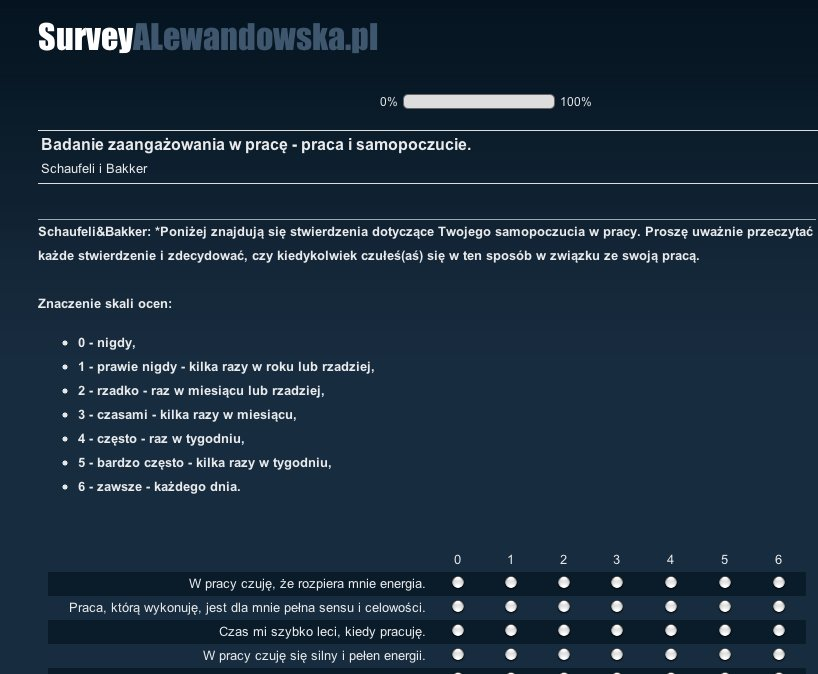
\includegraphics[width=0.8\textwidth]{survey}
\end{center}
\caption{Wygląd pierwszej strony ankiety internetowej z pytaniami.}
\label{fig:sex}
\end{figure}

Odnośnik do gotowej ankiety internetowej został rozesłany drogą emaliową na listy emaliowe kilku instytucji i organizacji, w tym:
\begin{itemize}
\item na listę absolwentów kierunku Informatyka na Wydziale Informatyki i Zarządzania Politechniki Poznańskiej -- rok ukończenia 2008,
\item na listę pracowników Poznańskiego Centrum Superkomputerowo-Sieciowego,
\item na listę pracowników Allegro.
\end{itemize}
Oczywiście wszyscy byli zachęcani do rozsyłania ankiety dalej, więc osoby biorące udział w badaniu nie muszą, ale mogą być ograniczone tylko do wskazanych firm. Wypełnienie ankiety było dobrowolne, przy czym wszystkie pytania w ankiecie były obowiązkowe, także dotyczące danych demograficznych.

\graphicspath{{img/group/}}
\section{Charakterystyka próby badawczej}

\graphicspath{{img/results/}}
\section{Opracowane wyników}

\subsection{Job Satisfaction Survey}

\begin{figure}[h]
    \centering
    \subfloat[Płaca]{\label{fig:his-pay}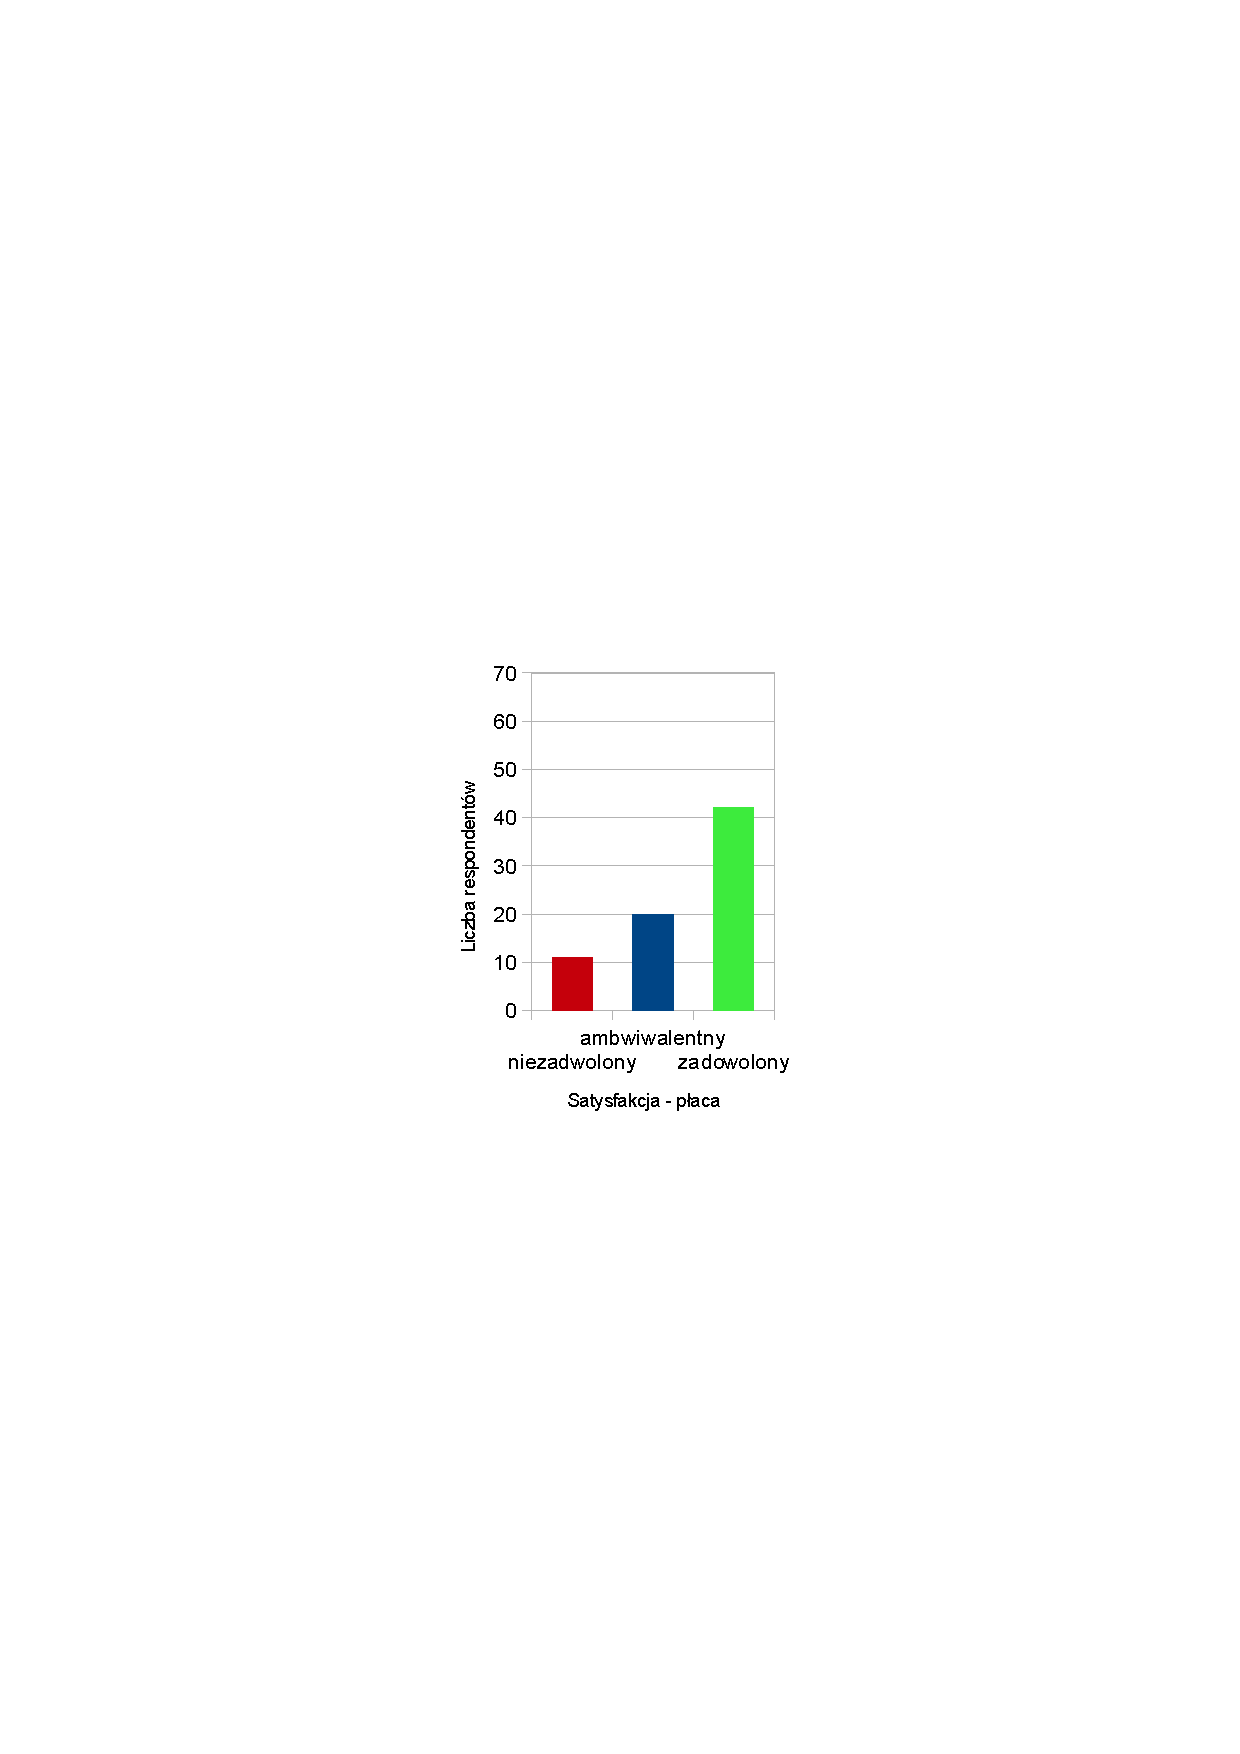
\includegraphics[height=0.27\textheight]{sat-pay}}
    \subfloat[Awanse]{\label{fig:his-promotion}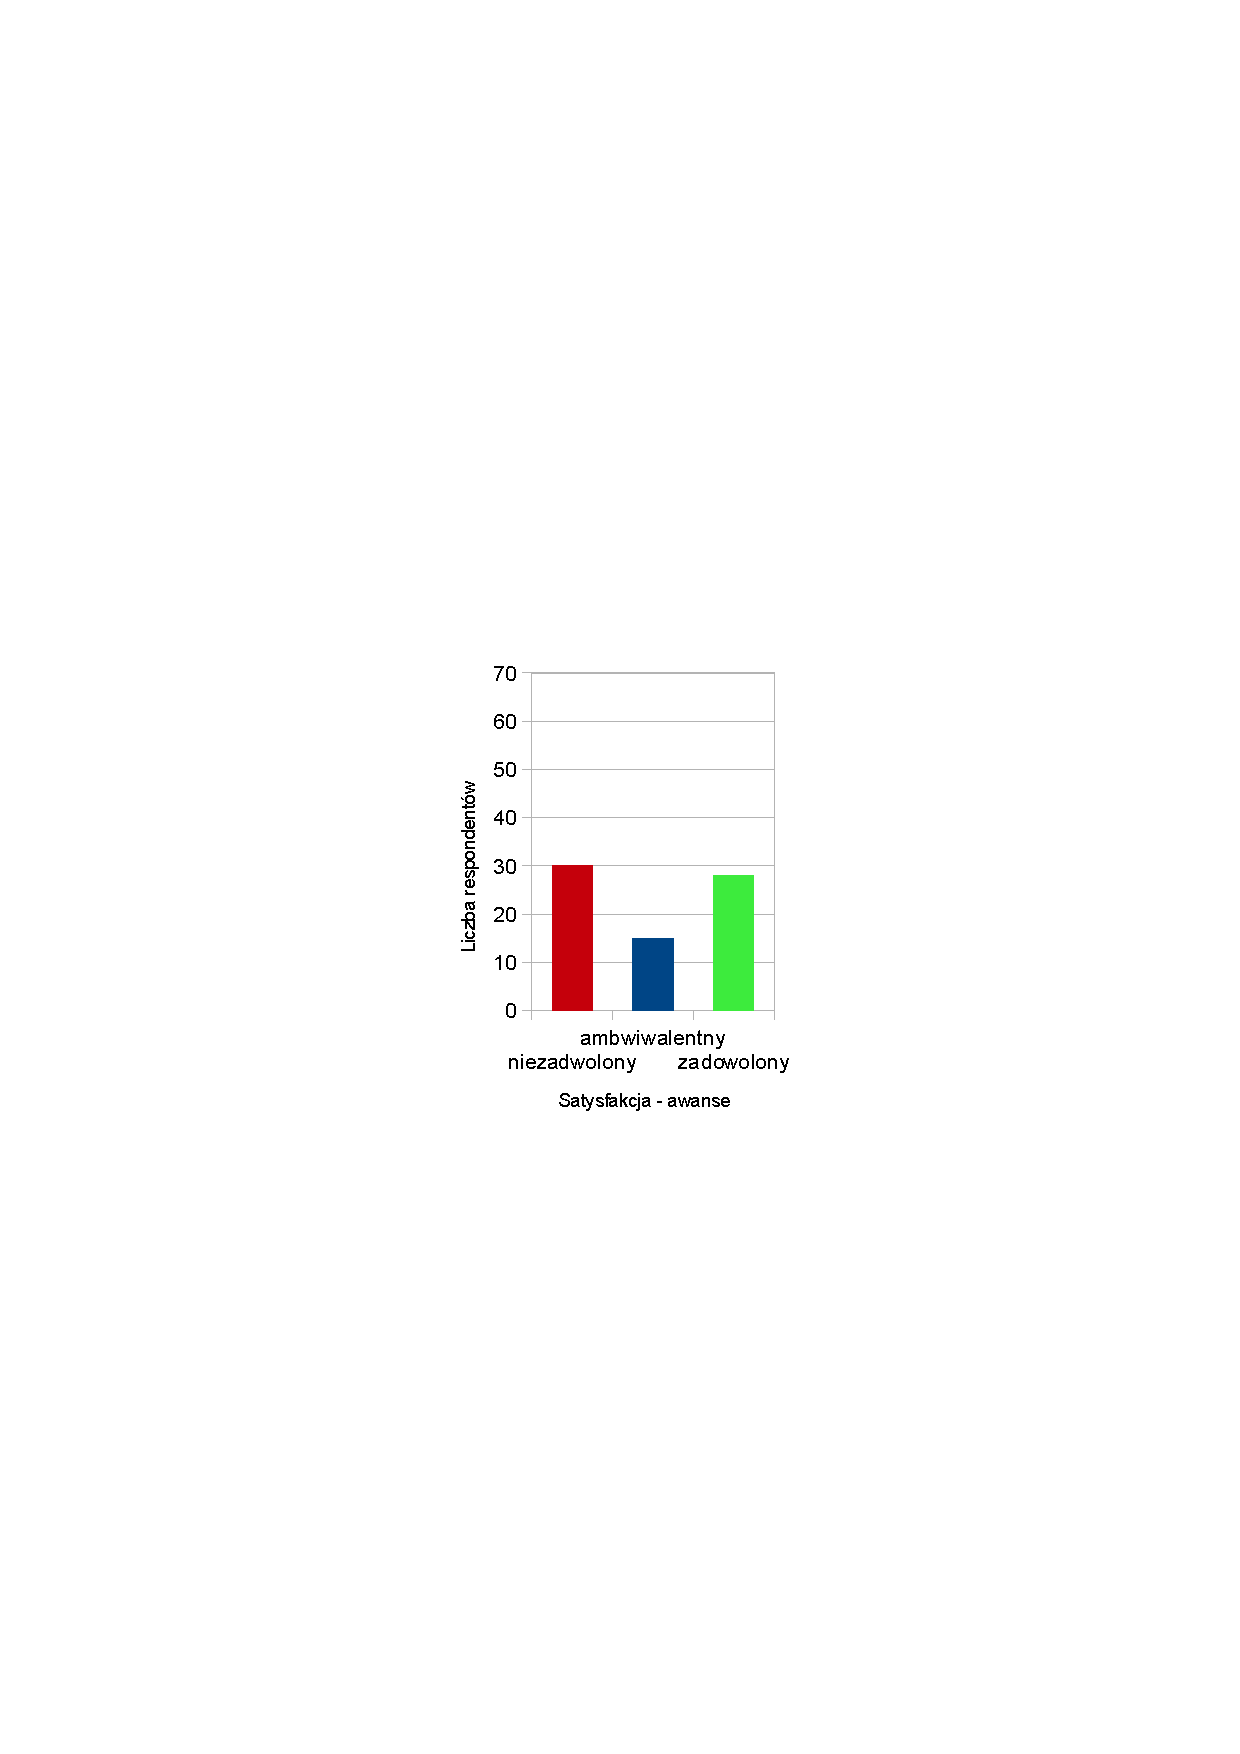
\includegraphics[height=0.27\textheight]{sat-promotion}}
    \\
    \subfloat[Nadzór]{\label{fig:his-supervision}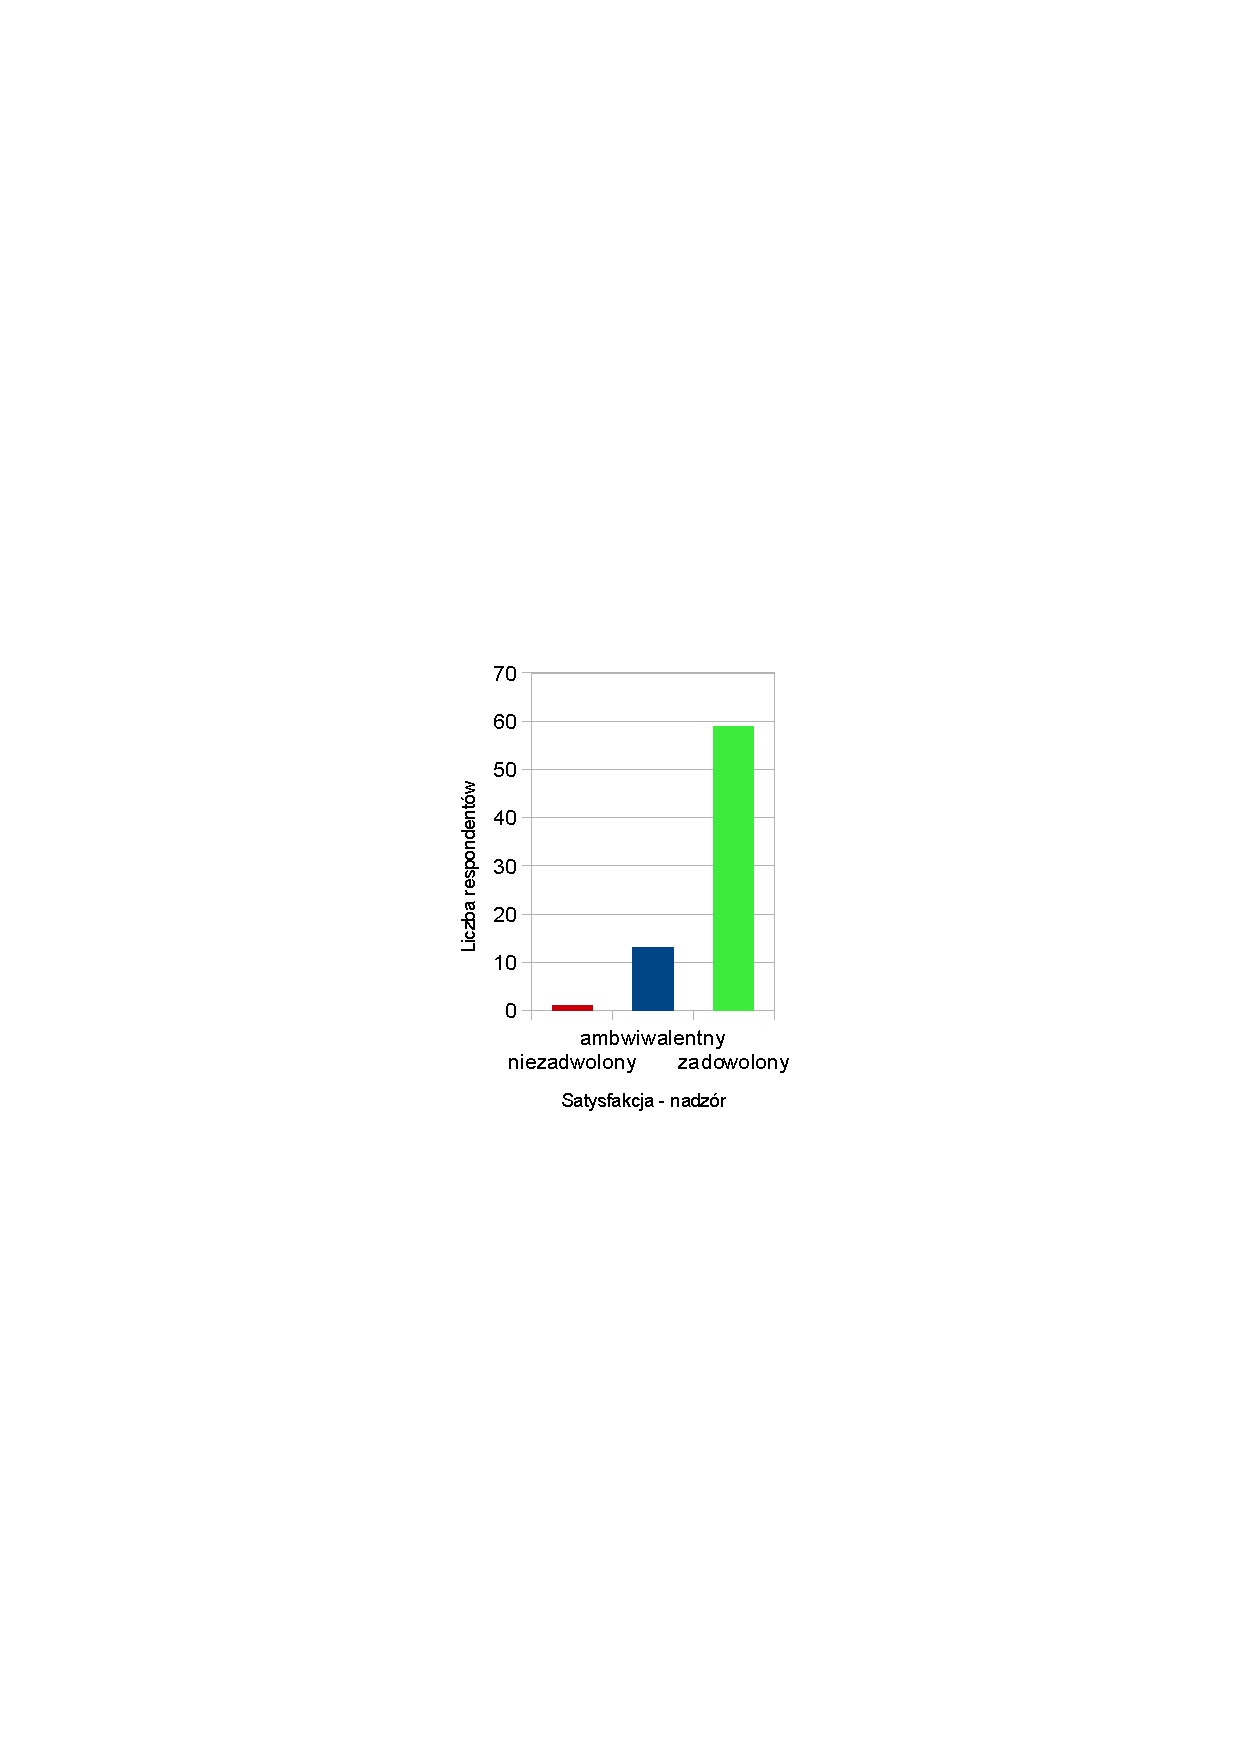
\includegraphics[height=0.27\textheight]{sat-supervision}}
    \subfloat[Dodatki]{\label{fig:his-benefits}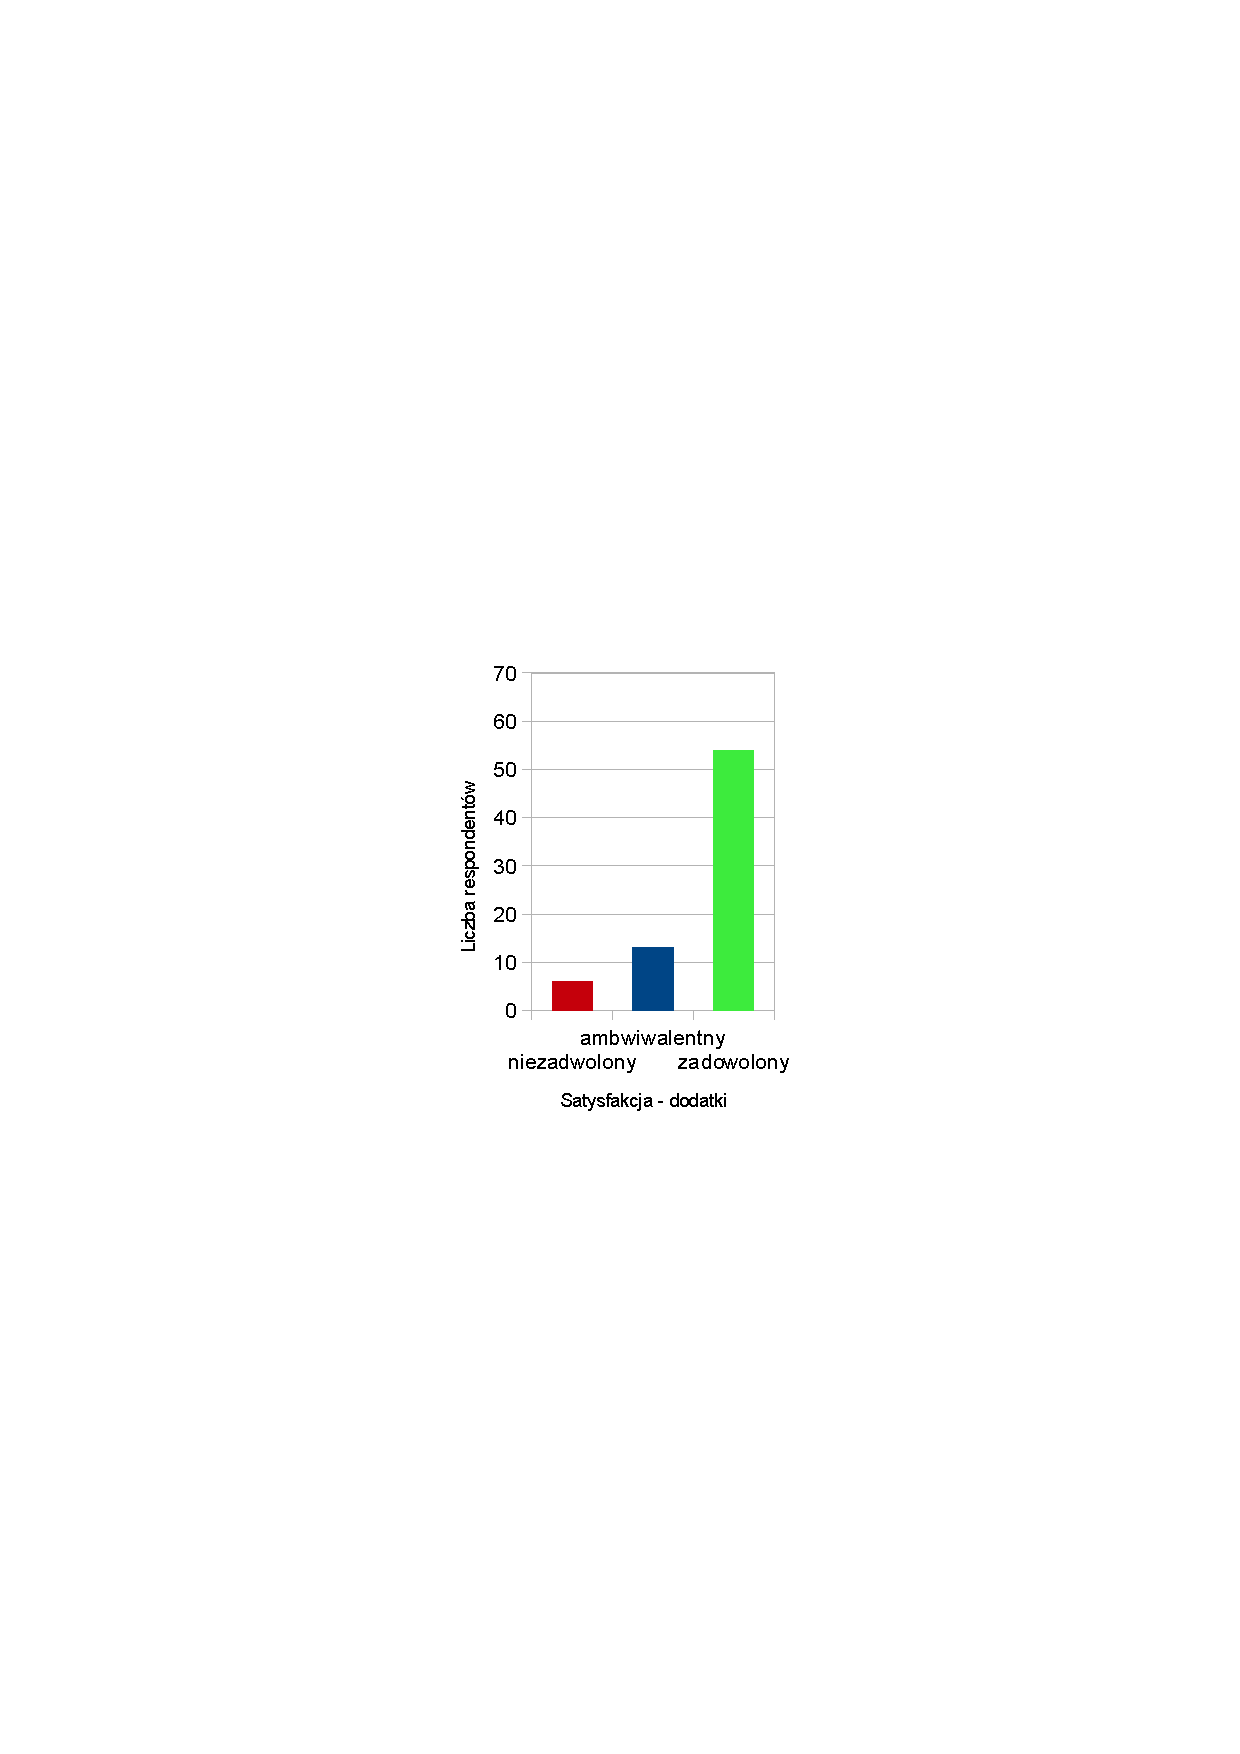
\includegraphics[height=0.27\textheight]{sat-benefits}}
    \\
    \subfloat[Nagrody]{\label{fig:his-rewards}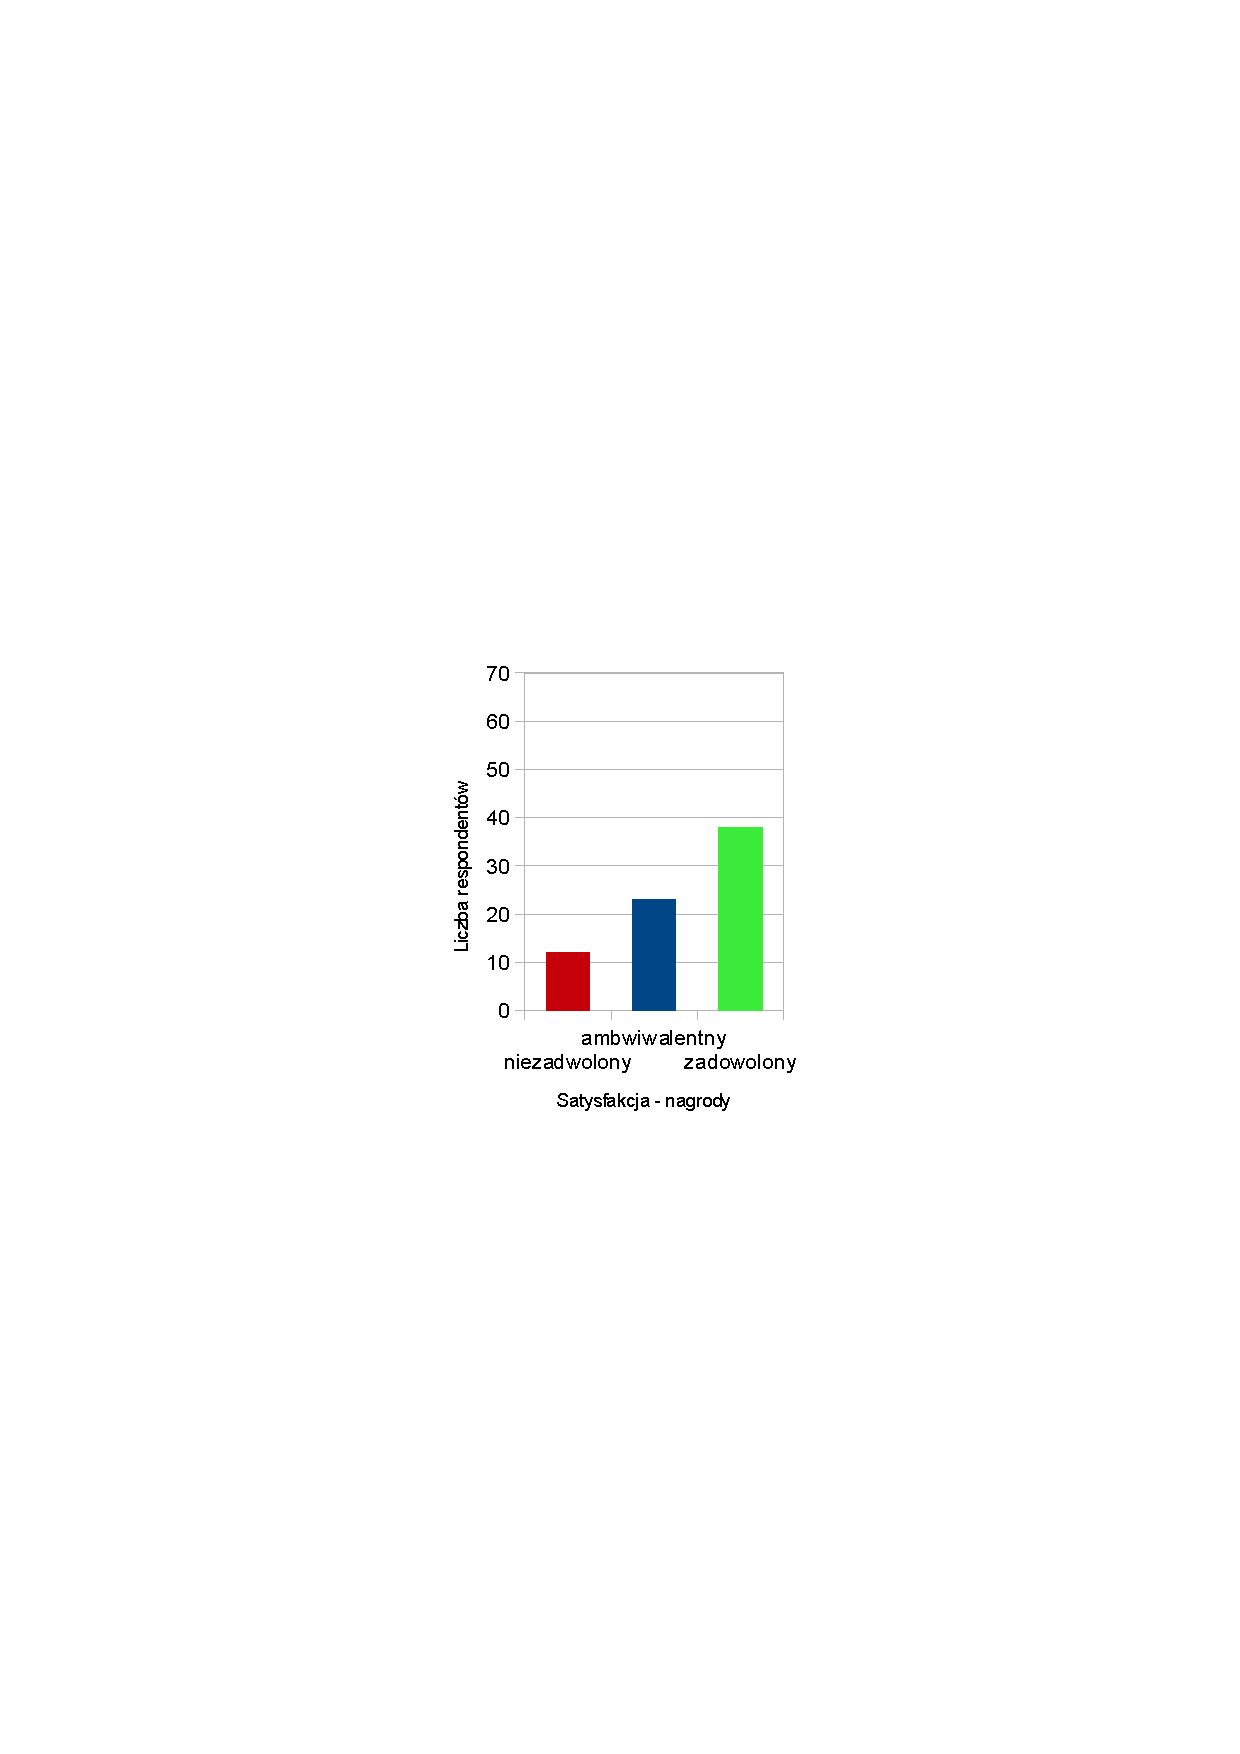
\includegraphics[height=0.27\textheight]{sat-rewards}}
    \subfloat[Warunki]{\label{fig:his-conditions}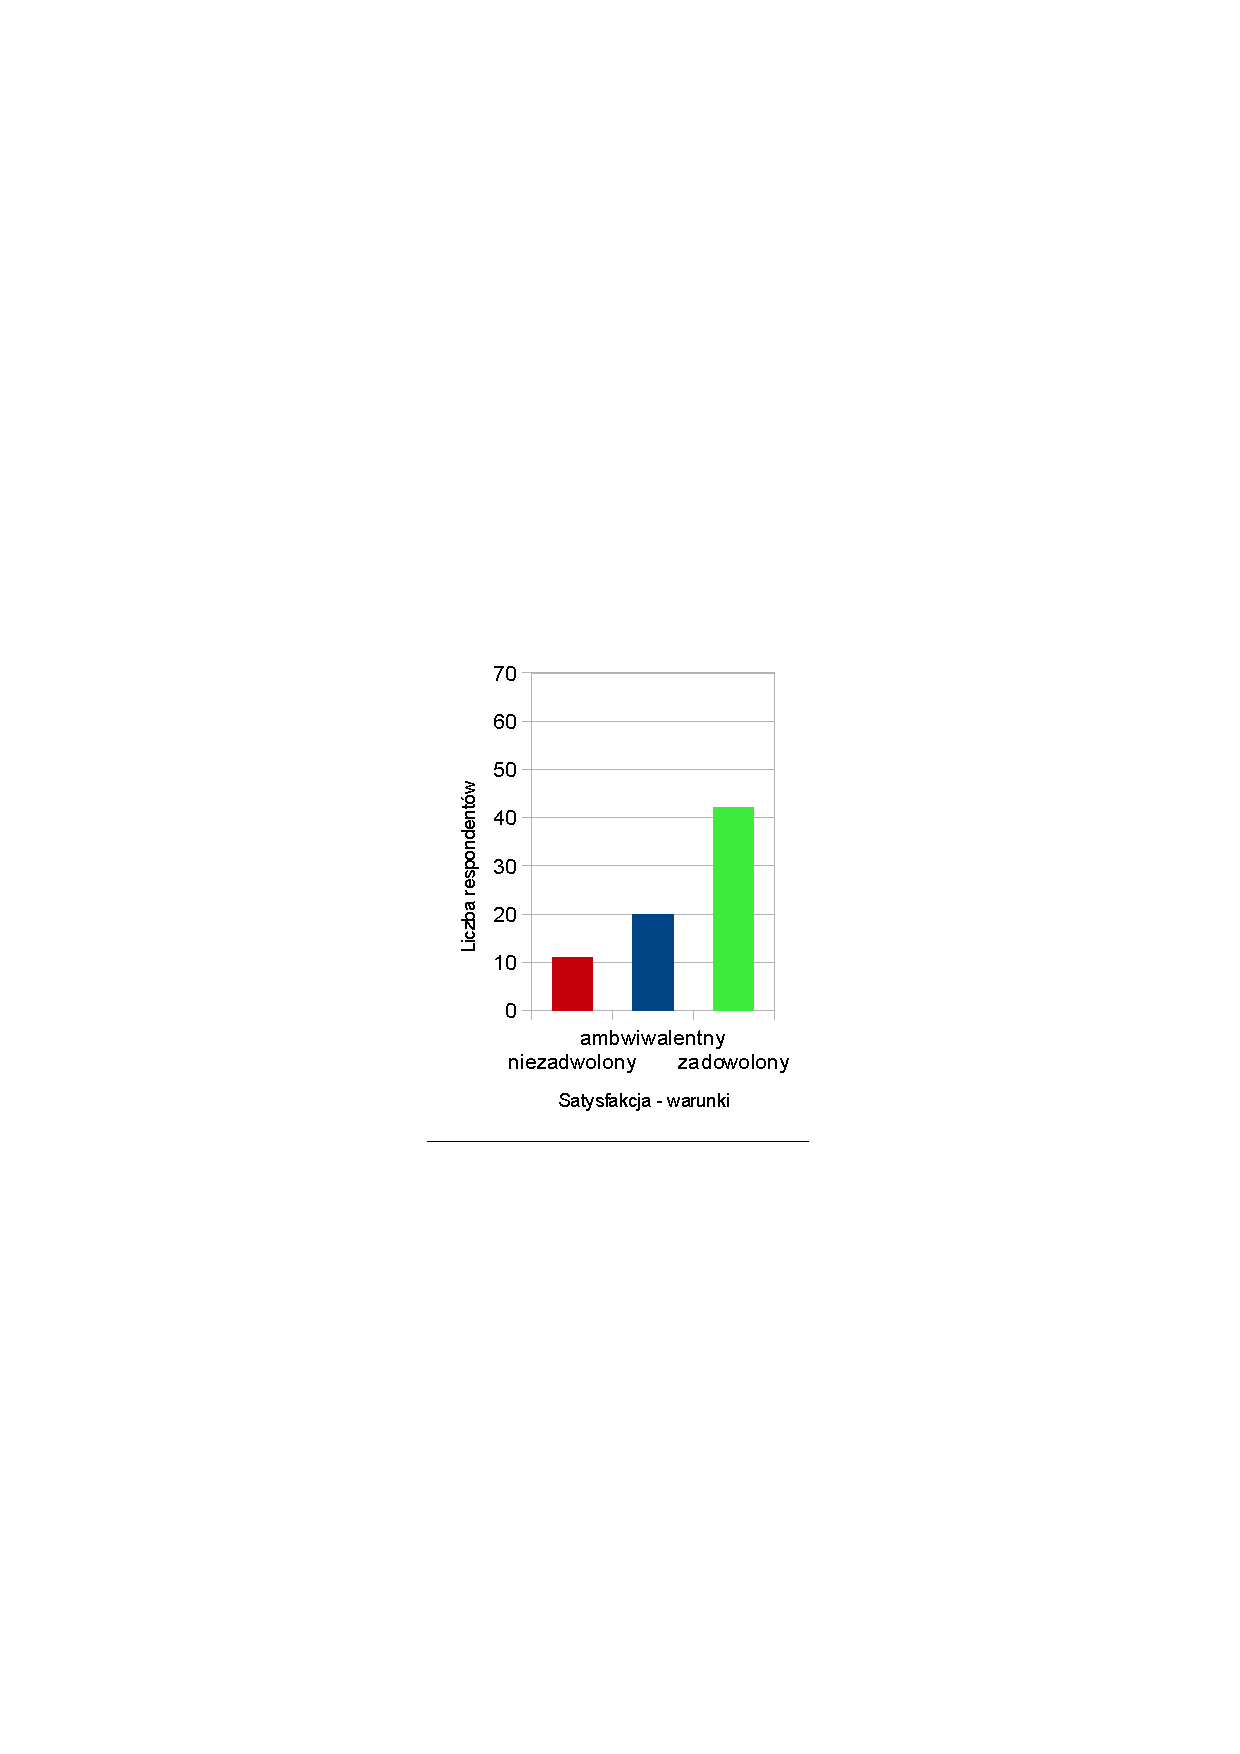
\includegraphics[height=0.27\textheight]{sat-conditions}}
    \caption{Histogramy dla \emph{JSS} -- część pierwsza}
\end{figure}

\begin{figure}[h]
    \centering
    \subfloat[Współpracownicy]{\label{fig:his-pay}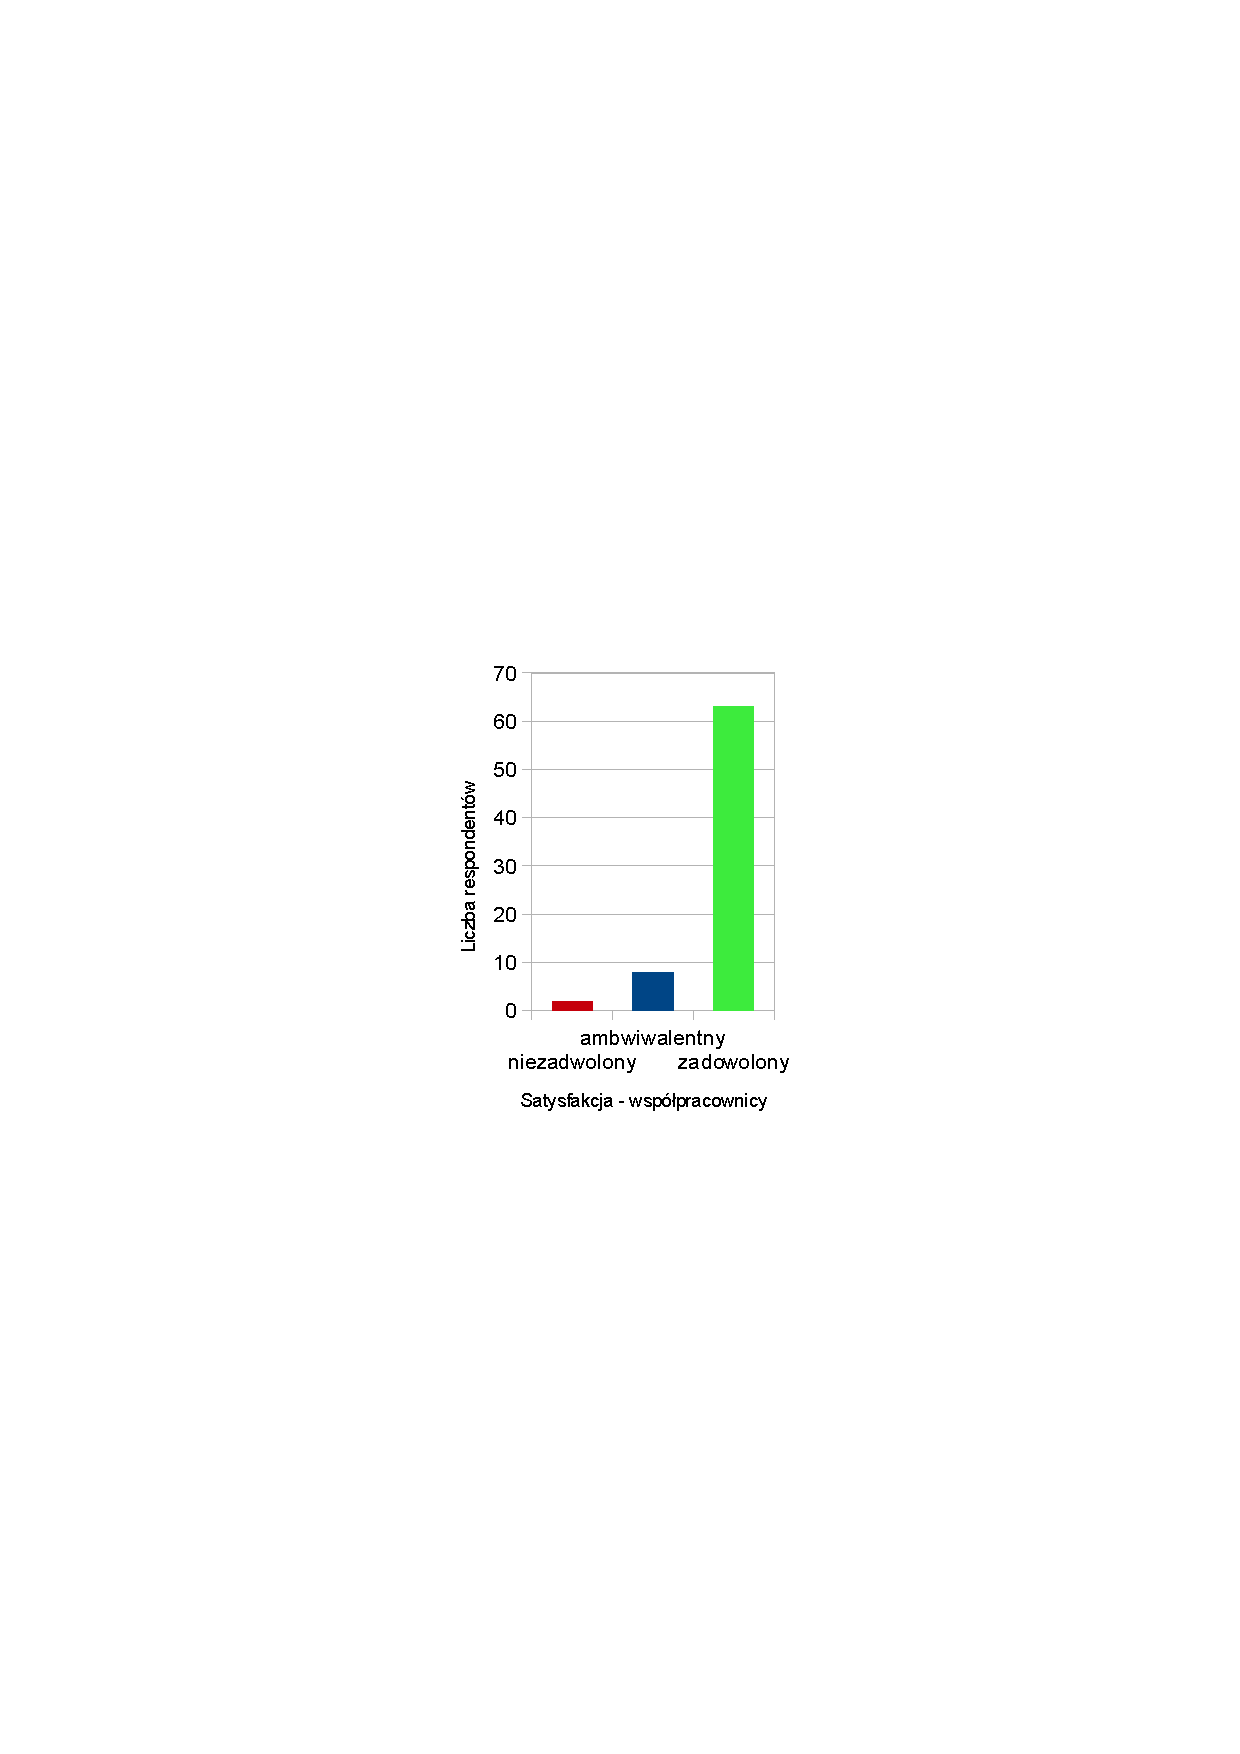
\includegraphics[height=0.27\textheight]{sat-coworkers}}
f   \subfloat[Wykonywana praca]{\label{fig:his-promotion}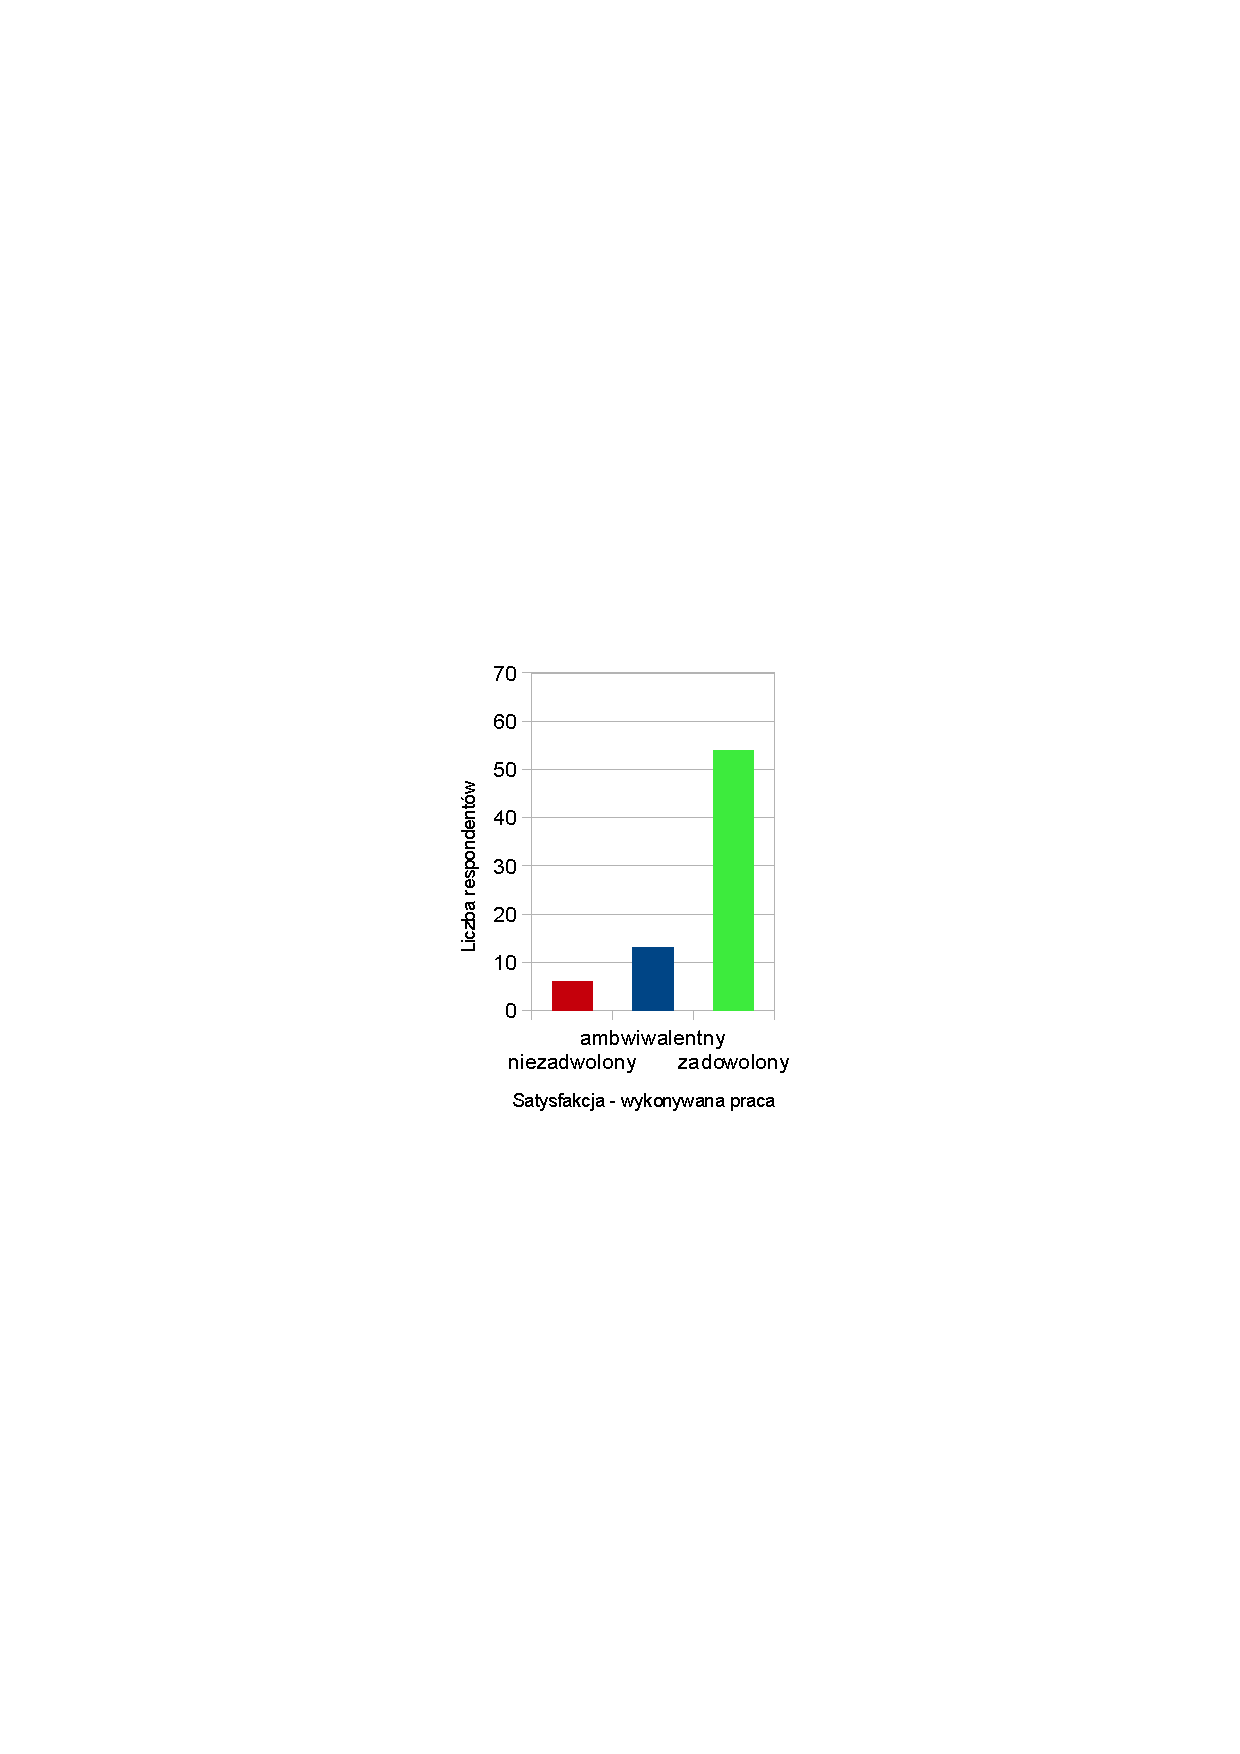
\includegraphics[height=0.27\textheight]{sat-work}}
    \\
    \subfloat[Komunikacja]{\label{fig:his-pay}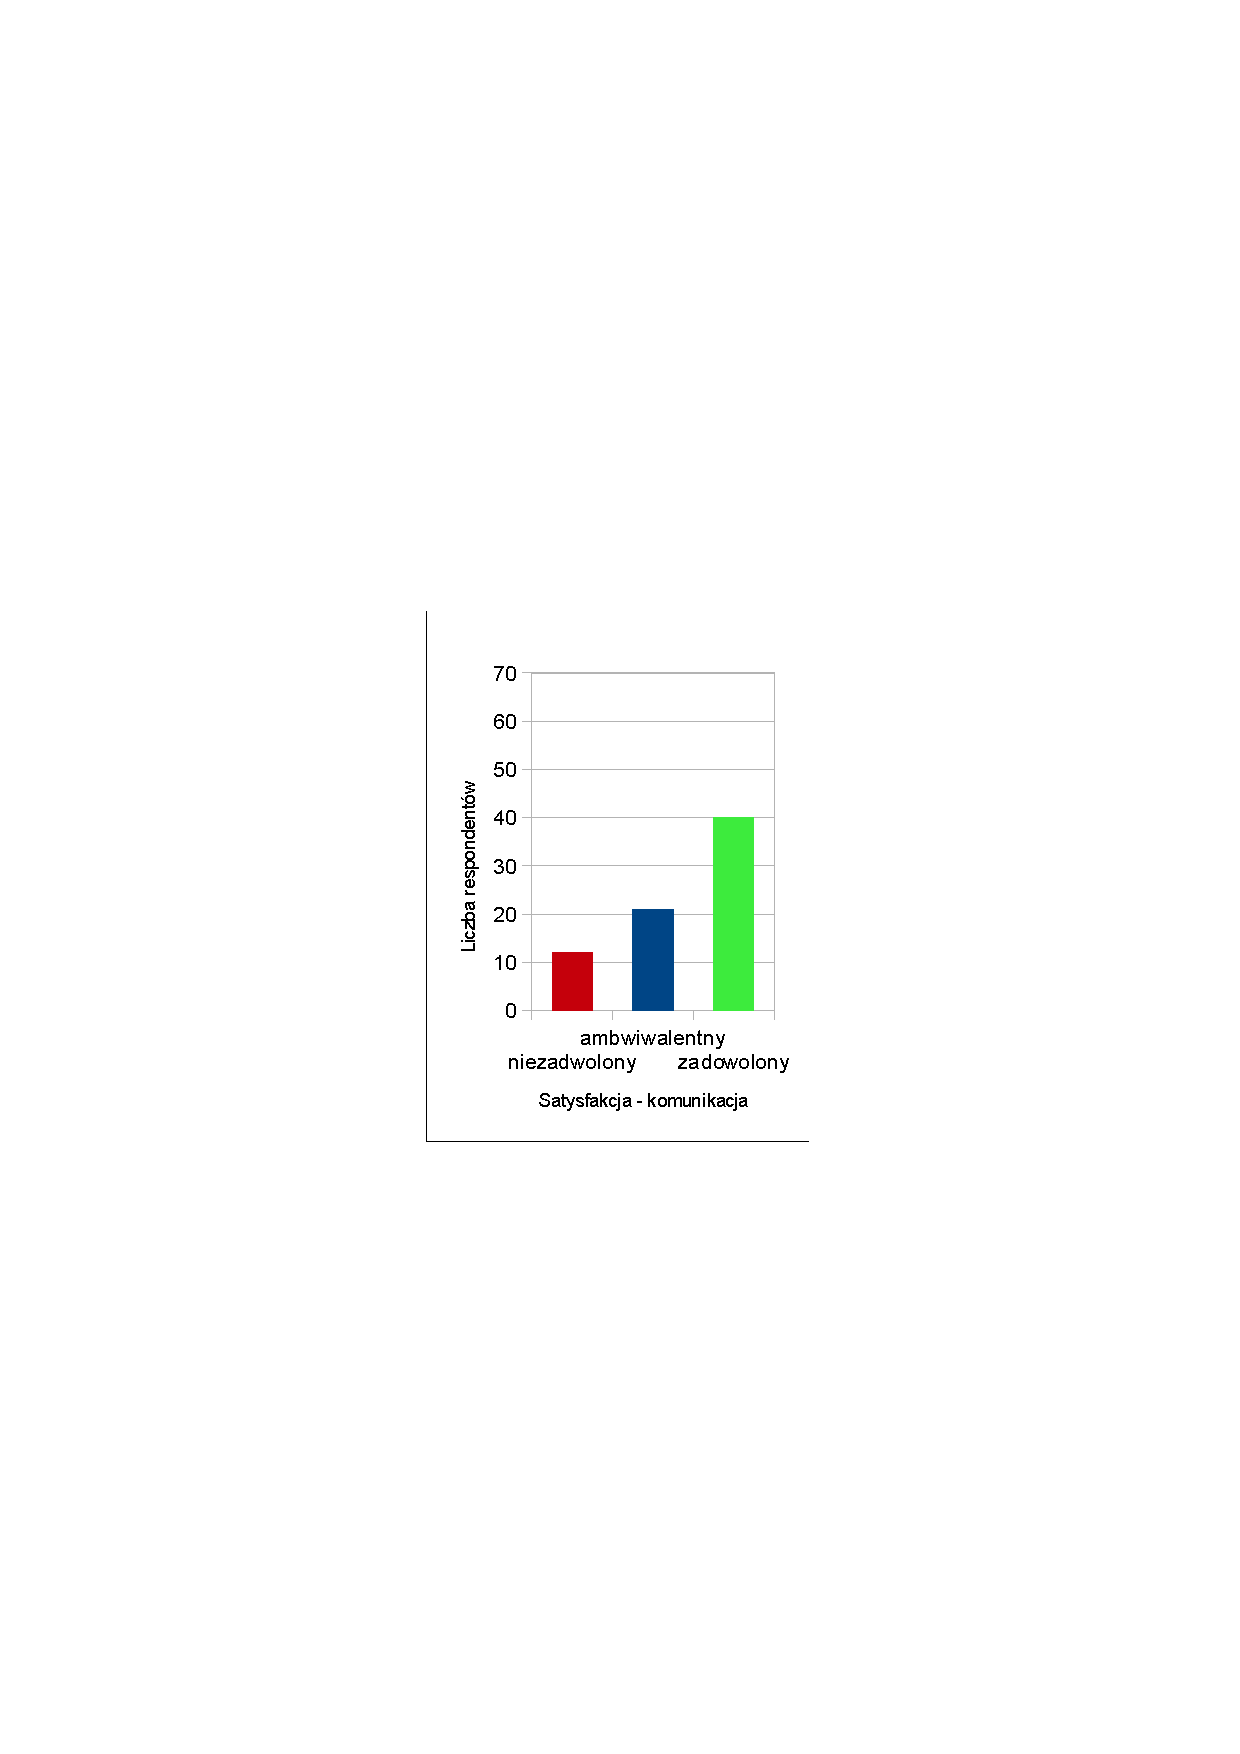
\includegraphics[height=0.27\textheight]{sat-communication}}
    \subfloat[Satysfkacja]{\label{fig:his-promotion}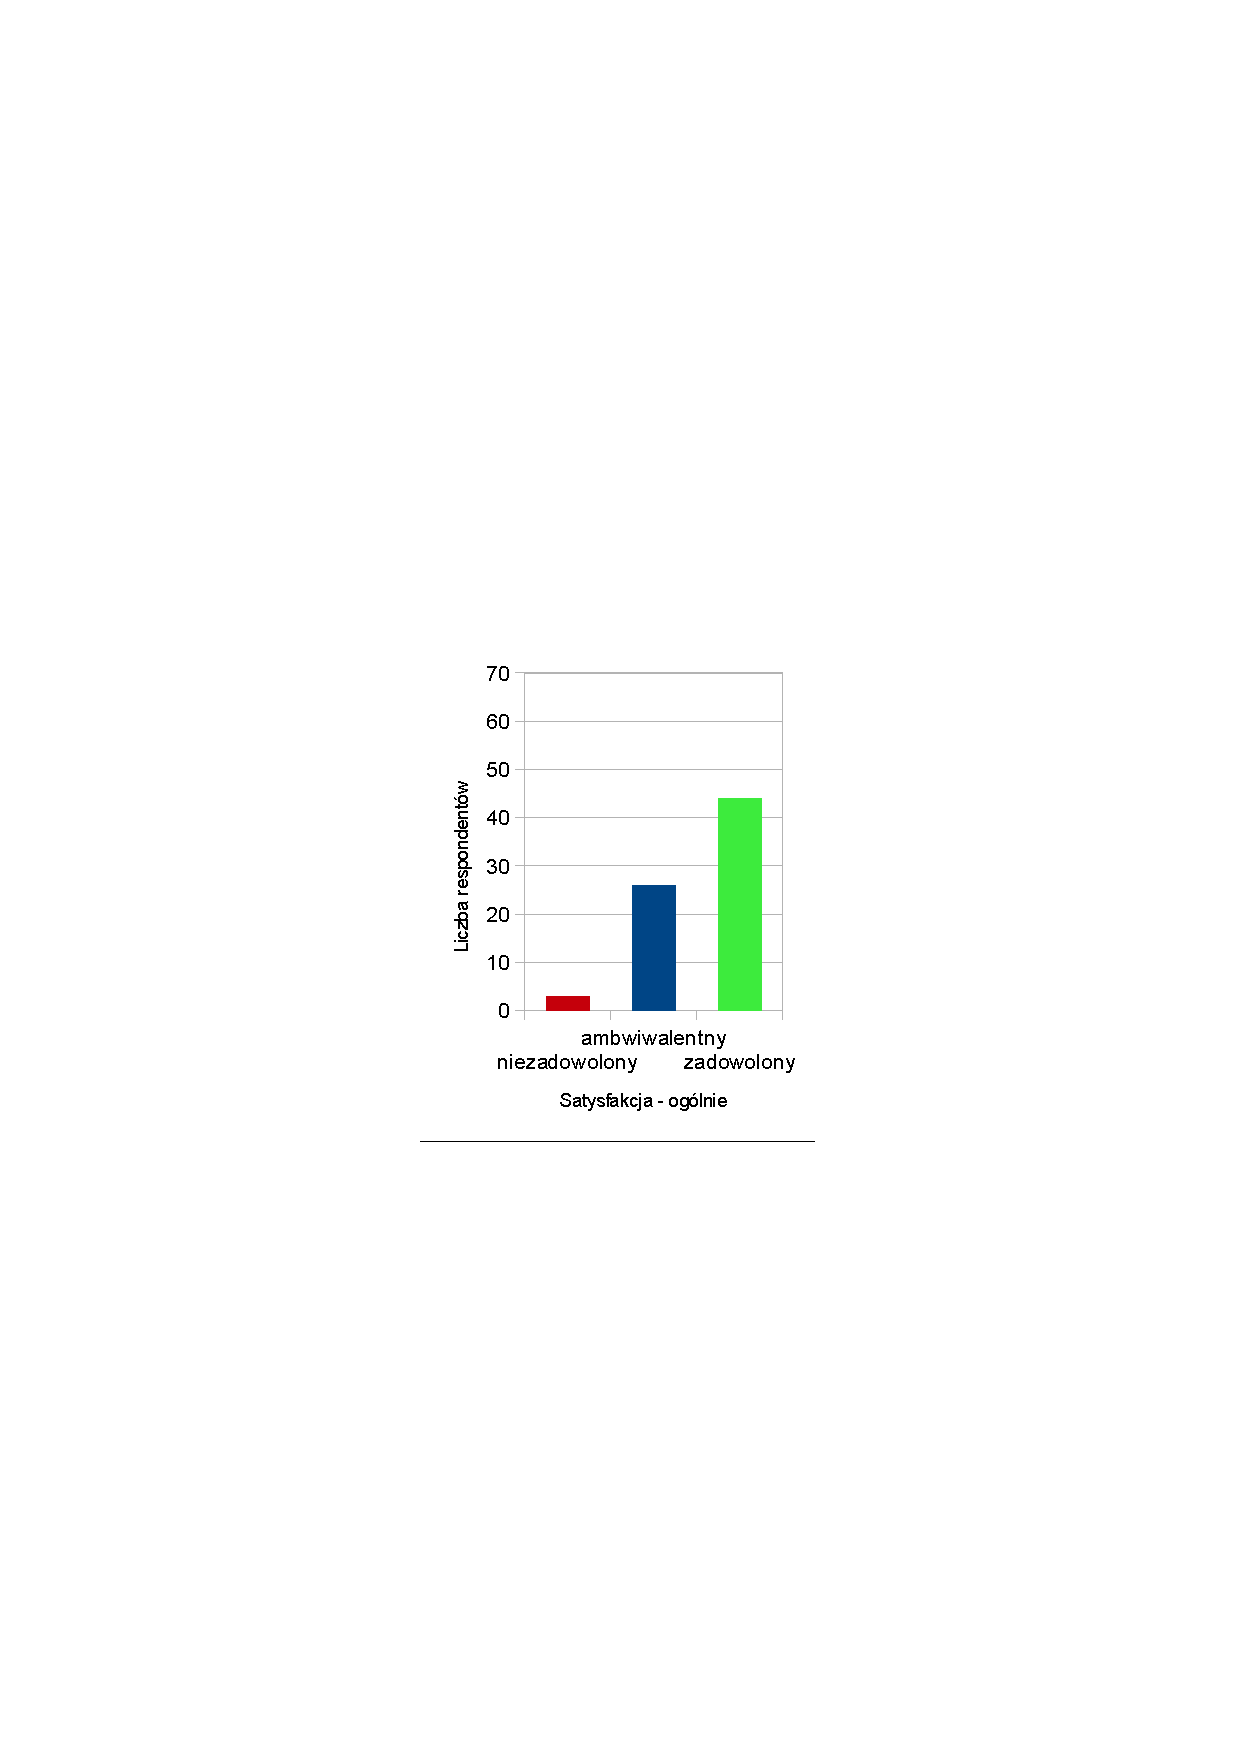
\includegraphics[height=0.27\textheight]{sat}}
    \caption{Histogramy dla \emph{JSS} -- część druga}
\end{figure}

\begin{table}[h!]
\begin{center}
\begin{tabular}{l | c c c c c c c c c c}
Wymiar & Min. & 1 kwartyl & Mediana & 3 kwartyl & Max.\\ \hline \hline
Płaca & 5 & 13 & 16 & 19 & 23 \\ 
Awanse & 4 & 10 & 14 & 17 & 23 \\
Nadzór & 10 & 17 & 20 & 22 & 24 \\
Dodatki & 9 & 15 & 18 & 20 & 24 \\
Nagrody & 5 & 13 & 16 & 19 & 24 \\
Warunki & 5 & 12 & 16 & 18 & 24 \\
Współpracownicy & 10 & 17 & 20 & 21 & 24 \\
Wykonywana praca & 6 & 15 & 19 & 21 & 24 \\
Komunikacja & 6 & 12 & 16 & 19 & 24 \\ \hline
Satysfakcja & 98 & 126 & 154 & 170 & 202 \\ \hline
\end{tabular}
\end{center}
\caption{Statystyki \emph{JSS} -- część pierwsza.}
\label{tab:jss-stats-1}
\end{table}

\begin{table}[h!]
\begin{center}
\begin{tabular}{l | c c c c c c c c c c}
Wymiar & Średnia & Moda & Wariancja & Odch. std. & Alfa Cronbacha\\ \hline \hline
Płaca & 15,99 & 19 & 18,57 & 4,31 & 0,77 \\
Awanse & 13,47 & 11 & 25,61 & 5,06 & 0,84 \\
Nadzór & 19,18 & 23 & 13,98 & 3,74 & 0,68 \\
Dodatki & 17,19 & 16 & 13,02 & 3,61 & 0,54 \\
Nagrody & 15,86 & 19 & 20,68 & 4,55 & 0,76 \\
Warunki & 15,51 & 16 & 17,5 & 4,18 & 0,59 \\
Współpracownicy & 19,08 & 20 & 9,35 & 3,06 & 0,58 \\
Wykonywana praca & 17,75 & 19 & 17,77 & 4,22 & 0,82 \\
Komunikacja & 15,62 & 12 & 18,27 & 4,27 & 0,67 \\ \hline
Satysfakcja & 149,64 & 125 & 645,51 & 25,41 & 0,91 \\ \hline
\end{tabular}
\end{center}
\caption{Statystyki \emph{JSS} -- część druga.}
\label{tab:jss-stats-2}
\end{table}

\begin{table}[h!]
\begin{center}
\begin{tabular} { l | c c c c c c c c c }
 & Pła & Awa & Nad & Dod & Nag & War & Wsp & Wp & Kom \\ \hline \hline
Pła & --- & 0,44 & 0,42 & 0,62 & 0,64 & 0,33 & 0,25 & 0,45 & 0,3 \\
Awa & & --- & 0,28 & 0,46 & 0,54 & 0,33 & 0,22 & 0,38 & 0,45 \\
Nad & & & --- & 0,49 & 0,58 & 0,28 & 0,41 & 0,47 & 0,38 \\
Dod & & & & --- & 0,66 & 0,38 & 0,34 & 0,46 & 0,32 \\
Nag & & & & & --- & 0,43 & 0,49 & 0,49 & 0,44 \\
War & & & & & & --- & 0,12 & -0,01 & 0,43 \\
Wsp & & & & & & & --- & 0,43 & 0,32 \\
Wp & & & & & & & & --- & 0,37 \\
Kom & & & & & & & & & ---  \\
\end{tabular}
\end{center}
\caption[Korelacja dla wszystkich wymiarów \emph{JSS}]{Korelacja dla wszystkich wymiarów \emph{JSS} (Pła -- Płaca, Awa -- Awanse, Nad -- Nadzór, Dod -- Dodatki, Nag -- Nagrody, War -- Warunki, Wsp -- Współpracownicy, Wp -- Wykonywana praca, Kom -- Komunikacja)}
\label{tab:jss-correl}
\end{table}

\paragraph{Płaca.} Na podstawie tabel \ref{tab:jss-stats-1} oraz \ref{tab:jss-stats-2} można ocenić, że wyniki rozpościerają się od 5 do 23, czyli pokrywają prawie całą skalę wartośći (oprócz wartości granicznych skali). Co ciekawe, mediana (wartość 16) oraz wartość średnia (15,99) znajduje się dokładnie na granicy między ambwiwalentnym stosunkiem do płacy, a zadowoleniem. W związku z tym można stwierdzić, że ok. połowa pracowników sektora IT jest zadowolona ze swojej pracy. Odchylenie standardowe 4,31 na pięciostopniowej skali nie jest ani duże ani małe. Wskazuje
jednak na średnie wachania w danych. Z zadowalających rzeczy, alfa Cronbacha jest powyżej 0,7 (dokładnie 0,77) co wskazuję na spójność odpowiedzi w ramach wymiaru.

Patrząc na Tabelę \ref{tab:jss-correl} \textit{płaca} ma wysoki współczynnik korelacji z ogólną satysfakcją (dokładnie 0,73). Co było do przewidzenia, najniższa korelacja istnieje dla czynników pozafinansowych, społecznych: \emph{współpracowników} oraz \emph{komunikacji}

\paragraph{Awans.} Podobnie jak z \textit{płacą}, wyniki dla \emph{awansu} rozpościerają się prawie na całej skali (oprócz wartości maksymalnej dla skali). Pierwszy kwartyl i mediana znajduą się na poziomie niezadowolenia i niepewnego stosunku do tego aspektu pracy. Trzeci kwartyl (wartość 17) jest tylko nieznacznie w przedziale zadowolenia. Widać to wyrażnie na histogramie \emph{awansu} (Rysunek \ref{fig:his-promotion}) -- ponad połowa osób nie jest zadowolona
z możliwości awansu w pracy. Dodatkowo odchylenie standardowe jest duże -- 5,06 i wskazuje na duży rozrzut w danych. Przy czym jest to wymiar satysfakcji, który jest najbardziej spójny jeżeli chodzi o odpowiedzni na zadane pytania. Uzyskał wynik 0,84 dla alfy Cronbacha.

Analizując Tabelę \ref{tab:jss-correl} widzimy, że najwyższa korelacja tego aspektu pracy jest z \textit{nagrodami}. Jednak jest to wartość nieznacznie powyżej 0,5 (dokładnie 0,54). W następnej kolejności są \emph{dodatki}. Jest to zgodne z formą przyznawania awansów i nagród, są to formy uznania przez przełożonego i podlegją jego subiektywnej ocenie. Co ciekawe, z drugiej strony, korelacja z wymiarem oceny przełożonego (\emph{nadzór}) jest słaba. Wskazuje to na niesymetryczność w
ocenie na poziomie relacji szef-przełożony. Uzupełniając, z resztą wymiarów \textit{awans} jest słabo skorelowany. 

Ogólnie wyniki dla \textit{awansu} są najsłabsze w porównianiu z innymi wymiarami. Oznacza to, że jest to aspekt pracy, z której pracownicy są najmniej zadowoleni.

\paragraph{Nadzór.} Skala dla \textit{nadzoru} zaczyna się dopiero od wartości 10 i kończy na maksmalnej możliwej -- 24. Pierwszy kwartyl (wartość 17) znajduje się na poziomie satysfakcji z pracy, mediana to 20, a trzeci kwartyl to 22 (tylko dwa punkty przed końcem skali). Jeżeli dodamy do tego średnią na pizomie 19,18 oraz modę równą 23 widać wyraźnie, że większość respondentów jest bardzo zadowolonych ze swoich przełożonych. Widać to bardzo dobrze na histogramie na Rysunku
\ref{fig:his-supervision}. Dodatkowo w miarę niskie odchylenie standardowe
na poziomie 3,74 wskazuje na mały rozrzut wartości w danych. Co ciekawe alfa Cronbacha jest na granicy akceptowalności (TODO kto to wyznaczył -> znajdź w UWES)a i wynosi 0,68.

Natomiast w Tabeli \ref{tab:jss-correl} znajdują się korelacje między \textit{nadzorem}, a innymi wymiarami \textit{satysfakcji}. Najwyższa wartość jest powiązana z otrzymywanymi nagrodami (wymiar \textit{nagrody}) i wynosi 0,58 (czyli nieznacznie ponad 0,5 -- średniej siły korelacja). Oznacza to, że przełożonych doceniamy najbardziej za nagrody jakie od nich otrzymujemy, czyli dodatkowe formy uznania naszej pracy. Następnie w kolejności są \textit{dodatki} (0,49), a
później \textit(wykonywana praca) (0,47). Interesująca jest zależność z wykonywaną pracą, wskazuje to na docenienie szefa za zlecane zadania. Z drugiej strony, niska korelacja z wymiarem \textit{warunków} oraz \textit{komunikacji} wskazuje na oczekiwania jakie pracownicy stawiają swoim przełożonym. O dziwio nie wiążą się one z ułatwianiem pracy (np: warunki, które sprzyjają wydajnej pracy, jasno stawiane cele), chociaż takie teoretycznie powinny być m.in. wymagania wobec przełożonych.

\paragraph{Dodatki.}\label{par:res-benefits} Przyjmowane wartości przez ten wymiar zaczynają się dopiero od 9 i ciągną się do maksymalnej wartości. Pierwszy kwartyl jest blisko granicy między abwiwalentnymi odczuciami, a satysfakcją. Czyli ok. 75\% respondentów jest zadowolona ze swoich dodatków. Mediana (wartość 18), trzeci kwartyl (wartość 20) i średnia (wartość 3,61) znajdują się już w granicach pułapu dla określenia satysfakcji. Widać to bardzo ładnie na histogramie wartości na
Rysunku \ref{fig:his-benefits}. Jeżeli dodamy do tego dość niskie
odchylenie standardowe o wartości 3,61 widzimy, że respondenci są całkiem zgodni jeżeli chodzi o zadowolenie z otrzymywanych dodatków. Z drugiej strony Alfa Cronbacha jest najniższa ze wszystkich wymiarów i wynosi 0,54. Wskazuje to na najmniejszą spójność w odpowiedziach na pytania odnośnie dodatków w pracy.

Przyglądając się korelacji w Tabeli \ref{tab:jss-correl}, najwyższą wartość posiada z \textit{nagrodami} (wartość 0,66) oraz z \textit{płacą} (wartość 0,62). Jest to zgodne z założeniami, że jeżeli firmę stać na dodatki takie jak dodatkowy pakiet medyczny dla pracowników, posiada ona wysokie zasoby pienieżne, tak aby móc wypłacać wysokie pensje. Przyczyna ta może, ale nie musi, wiązać się z wypłacaniem nagród czy też ich rodzajem. 

\paragraph{Nagrody.} \textit{Nagrody} mają bardzo podobne statystyki co \textit{płace}. Minimalna wartość to 5, pierwszy kwartyl to 13, mediana (wartość 16) jest na granicy między ambwiwalentnym stosunkiem, a satysfakcją. Trzeci kwartyl to 19. Tylko wartość maksymalna jest o 1 większa i wynosi 24. Jeżeli dodamy do tego średnią na poziomie 15,86 (czyli granica między ambwiwalencją, a satysfakcją) i spojrzymy na histogram wartośći na Rysunku \ref{fig:his-rewards},
dostrzegamy, że ok. połowa badanych jest zadowolona z orzymywanych nagród, jedna-trzecia ma odczucia mieszane, reszta jest po prostu niezadowolona. Dodatkowo odchylenie standardowe jest na średnim poziomie i wynosi 4,55. Wskazuje to na średni rozrzut danych w odpowiedziach badanych. Za to alfa Cronbacha jest bardzo wysoka i wynosi 0,76 (powyżej granicy 0,7) i wskazuje na rzetelność tej skali.

Patrząc na Rysunek \ref{tab:jss-correl} widzimy korelacje dla \textit{nagród}. Najzwyższa jest z \textit{dodatkami} oraz z \textit{płacą}. Możliwe przyczyny zostały już opisywane w paragrafie wyżej nt \textbf{dodatków} (sekcja \ref{par:res-benefits}). Wysoka korelacja jest także z \textit{awansami} (wartość 0,54) oraz \textit{nadzorem} (wartość 0,58). \textit{Awanse} mogą się wiązać z podobieństwiem przyczyny otrzymywania \textit{nagród} i \textit{awansów} -- jest to forma
docenienia dobrej pracy pracownika. Czyli pracownicy, którzy dostają dużo nagród są brani pod uwagę przy awansach i prawdopodobnie szybciej pną się po szczeblach kariery. Natomiast co do \textit{nadzoru} wydaje się to być naturalnym, że mamy pozytywny stosunek do osób, które w jakiś sposób nas doceniają.

\paragraph{Warunki.} Skala dla warunków rozciąga się od prawie minimalnej wartości (5) do maksymalnej możliwej (24). Pierwszy kwartyl (wartość 12) znajduje się na granicy niezadowolenia i niepewnych odczuć, co oznacza, że mniej niż 25\% pracowników nie odczuwa satysfakcji z pracy. Mediana (wartość 16) jest na granicy między mieszanymi odczuciami, a zadowoleniem z pracy (podobnie jak średnia -- 15,51) -- co oznacza razem z pierwszy kwartylem ponad 25\% ambwiwalentnych. Trzeci kwartyl (wartość 18) to już zadowlenie, czyli ok. 50\% jest zadowolonych ze swoich
warunków z pracy. Potwierdza to wykres histogramu na Rysunku \ref{fig:his-conditions}. Wariancja jest średnio wysoka i wynosi 4,18. Wskazuje to na w miarę duże różnice w odpowiedziach respondentów. Natomiast co do rzetelności skali, to alfa Cronbacha jest powyżej progu 0,7 i wynosi 0,76 co wskazuje na spójne odpowiadanie na zadane pytania.

Przechodząc do korelacji, \textit{warunki} posiadają najwyższą wartość dla tego współczynnika dla \textit{komunikacji} i \textit{nagród} -- oba wynoszą 0,43 (średnia korelacja). Jeżeli chodzi o \textit{nagrody} można to wytłumaczyć tym, że jeżeli firmę stać na pokrywanie zadowalających nagród dla pracowników, wówczas stać ich także na zapewnienie zadowalających warunków pracy. Za to ciekawa jest korelacja z \textit{komunikacją}. Możliwe, że jeżeli komunikacja w ramach firmy jest dobra, to informacje o niedociągnięciach w
środowisku pracy docierają do odopowiednich osób i dzięki temu warunki się poprawiają. 

\paragraph{Współpracownicy.} Minimalna wartość dla \textit{współpracowników} zaczyna się dopiero od 10 i rozciąga się do maksymalnej możliwej wartości. Pierwszy kwartyl to 17 (czyli już na poziomie zadowolenia z pracy), mediana to 20, a trzeci kwartyl to 21. Jeżeli dodamy do tego średnią na poziomie 19,08 oraz odchylenie standardowe najniższe ze wszystkich - 3,06, widzimy, że respondenci byli zgodni co do wysokiej opini na temat swoich współpracowników. Potwierdza to wykres
na Rysunku \ref{fig:his-coworkers}. Co ciekawe metryki te są bardzo podobne jak dla \textit{pracy}. Dodatkowo alfa Cronabach jest jedną z najniższych i wynosi 0,58. Wskazuje to na możliwą niespójność w odpowiedziach badanych między konkretnymi pytaniamia w ramach wymiaru.

Przechodząc do korelacji (patrz Tabela \ref{tab:jss-correl} widzimy, że najwyższa wartość jest dla \textit{nagród} (wartość 0,49), a następnie dla \textit{wykonywanej pracy} (wartość 0,43). Relacja o średniej sile z \textit{nagrodami} początkowa wydaje się zaskakujące. Możliwe, że przyczyną są warunki finansowe firmy, tzn. jeżeli organizację stać na przekazywanie pracownikom zadowalających nagród, to także stać ich na zatrudnianie bardzo dobrych pracowników z dostępnych
na rynku pracy. Natomiast zależność z \textit{wykonywaną pracą} może wiązać się z profesjonalizmem współpracowników. Ludzie lubią prace, które są dla nich łatwe do zrozumienia (dopasowane do ich umiejętności, tzw. odpowiedniość pracy). Dzięki swojemu wysokiemu poziomowi wiedzy są w stanie wesprzeć innych pracowników podczas pracy.

Warto podkreślić, że jest to wymiar, z którego najwięcej osób jest zadowolonych (ok. 90\% respondentów).

\paragraph{Wykonywana praca.} Wyniki dla tego wymiaru rozpościerają się prawie na całej skali oprócz pierwszych dwóch najniższych wartośći. Pierwszy kwartyl (wartość 15) znajduje się na poziomie mieszanych uczuć, co oznacza, że co najmniej 25\% osób jest niezadowolonych lub nie jest pewnych swoich odczuć do wykonywanych zadań. Mediana (wartość 19) znajduje się już na poziomie zadowolenia, tak samo jak trzeci kwartyl (wartość 21). Czyli co najmniej 50\% respondentów jest zadowolonych z
natury ich pracy. Dane te potwierdza histogram na Rysunku \ref{fig:his-work}. Dodatkowo rozrzut odpowiedzi uczestników jest średniej wielkość (odchylenie standardowe to 4,22). Natomiast spójność skali jest bardzo wysoka (alfa Cronbacha 0,82).

Co do korelacji z Tabeli \ref{tab:jss-correl} \textit{wykonywana praca} najwyższą wartość ma dla \textit{nagród} (wartość 0,49), następnie \textit{nadzoru} (wartość 0,47) oraz \textit{dodatków} (wartość 0,46). \textit{Nagrody} oraz \textit{nadzór} można wiązać się z dobrym wykonywaniem zleconej pracy. Wiąże się to z otrzymywaniem nagród uznaniowych oraz chwaleniem przez przełożónych. Natomiast w wypadku \textit{dodatków} zależność może być w drugą stronę, tzn. miejsce pracy, które udostępnia swoich
pracowników dodatki (np.: karnet na siłownie) przyciąga bardziej zdolne osoby z rynku pracy, które lubią to co robią i robią to dobrze.

\paragraph{Komunikacja.} Wartości dla komunikacji rozciągają się od 6 do 24 (prawie cała skala). Pierwszy kwartyl (wartość 12) znajduje się na granicy między satysfakcją, a mieszanymi odczuciami. Mediana znajduje się na poziomie 16, czyli na granicy między ambwiwalencją, a zadowoleniem. Wynika z tego, że trochę mniej niż 25\% respondentów nie jest zadowolonych z tego aspektu swojej pracy i mniej więcej tyle samo ma ambwiwalentne uczucia. Trzeci kwartyl na poziomie 19 to
już zadowolenie z pracy. Czyli trochę ponad 50\% respondentów jest usatysfakcjonowanych komunikacją w miejscu pracy. Przyglądając się histogramowi z Rysunku \ref{fig:his-communication} widzimy, że osób niezadowolonych (12 osób, ok. jedna-szósta badanych) jednak jest o połowę mniej niż z mieszanymi odczuciami (21 osób, ok. jedna-trzecia badanych). Co ciekawe moda jest na wartośći 12, czyli granicznej między brakiem zadowolenia, a mieszanymi odczuciami. Jeżeli założymy, że 12 to jeszcze przedział
niezadowolenia wyniki wyglądają następująco: niezadowolenie -- 22 osoby, abwiwalencja -- 11 osóbk, czyli praktycznie na odwrót. W tym przypadku widzimy, jak delikatną sprawą jest określenie granic przedziałów i jak mogą one wpływać na końcową interpretację. Dlatego warto patrzeć na wszystkie miary statystyczne odnośnie danyhc (w tym przypadku medianę). 

Rozrzut odpowiedzi badanych był średnio wysoki, odchylenie standardowe wynosi 4,27. Natomiast alfa Cronbacha na poziomie 0,67 znajduje się na granicy 0,7 i można przyjąć, że skala ta jest skalą spójną (tzn. respondenci odpowiadali spójnie na pytania w ramach tej skali).

Patrząc dalej na Tabelę \ref{tab:jss-correl} z korelacjami, \textit{komunikacja} najwyższą zależność ma z \textit{awansami} (wartość 0,45), następnie istnieje zależność z \textit{nagrodami} (wartość 0,44). Jeżeli osoba jasno rozumie cele firmy, jest w stanie je realizować dobrze, a co za tym idzie spełniać oczekiwania i być promowanym oraz otrzymywać nagrody. Zbliżoną wartość mają także \textit{warunki} (wartość 0,43). Możliwe, że jasna komunikacja na linii
kierownictwo--przełożeni owocuje lepszym zrozumieniem potrzeb pracowników, a co za tym idzie także dostosowaniem warunków pracy do ich optymalnego wykonywania zadań.

\paragraph{Satysfakcja ogólna.}
Przymowane wartości rozciągają się od 98, do 202 (domena od 36 do 216). Dodając do tego pierwszy kwartyl (wartość 126) w granicach abwiwalentnych odczuć oraz medianę (wartość 154) oraz trzeci kwartyl (wartość 170), widzimy, że ponad 50\% respondentów jest zadowolonych ze swojej pracy. Średnia o wartośći 149,64 znajduje się także w przdziale zadowolenia. Dane te potwierdza histogram na Rysunku \ref{fig:his-sat}. Widzimy tam także, że osoby o mieszanych odczuciach to ok.
jedna-trzecia grupy, natomiast osoby niezadowolone całkowicie to znikoma ilość respondentów (dokładnie 3 osoby).

Odchylenie standardowe wynosi 25,41, czyli dla skali o szerorokości 180 jest to średnio-niski wynik, czyli średni rozrzut w danych. Natomiast alfa Cronbacha ma bardzo wysoki wynik i wynosi 0,91, co wskazuje na dużą spójność w odpowiedziach respondentów.
\subsection{Ultrech Work Engagement Survey}

\begin{table}[h!]
\begin{center}
\begin{tabular}{l | c c c c c c c c c c}
Wymiar & Min. & 1 kwartyl & Mediana & 3 kwartyl & Max.\\ \hline \hline
Wigor & 1,33 & 3 & 3,83 & 4,67 & 5,5 \\
Oddanie & 1,4 & 3 & 4 & 4,8 & 6 \\
Absorpcja & 1,17 & 3 & 3,5 & 4,67 & 5,83 \\ \hline
Zaangażowanie & 1,47 & 3 & 3,5 & 4,53 & 5,59 \\
\end{tabular}
\end{center}
\caption{Statystyki \emph{UWES} -- część pierwsza.}
\label{tab:uwes-stats-1}
\end{table}

\begin{table}[h!]
\begin{center}
\begin{tabular}{l | c c c c c c c c c c}
Wymiar & Średnia & Moda & Wariancja & Odch. std. & Alfa Cronbacha\\ \hline \hline
Wigor & 3,75 & 4 & 1,13 & 1,06 & 0,83 \\
Oddanie & 3,79 & 4,2 & 1,47 & 1,21 & 0,9 \\
Absorpcja & 3,76 & 4,67 & 1,21 & 1,1 & 0,86 \\ \hline
Zaangażowanie & 3,76 & 4,65 & 1,04 & 1,02 & 0,94 \\
\end{tabular}
\end{center}
\caption{Statystyki \emph{UWES} -- część druga.}
\label{tab:uwes-stats-2}
\end{table}

\begin{figure}[h]
    \centering
    \subfloat[Wigor]{\label{fig:eng-vigor}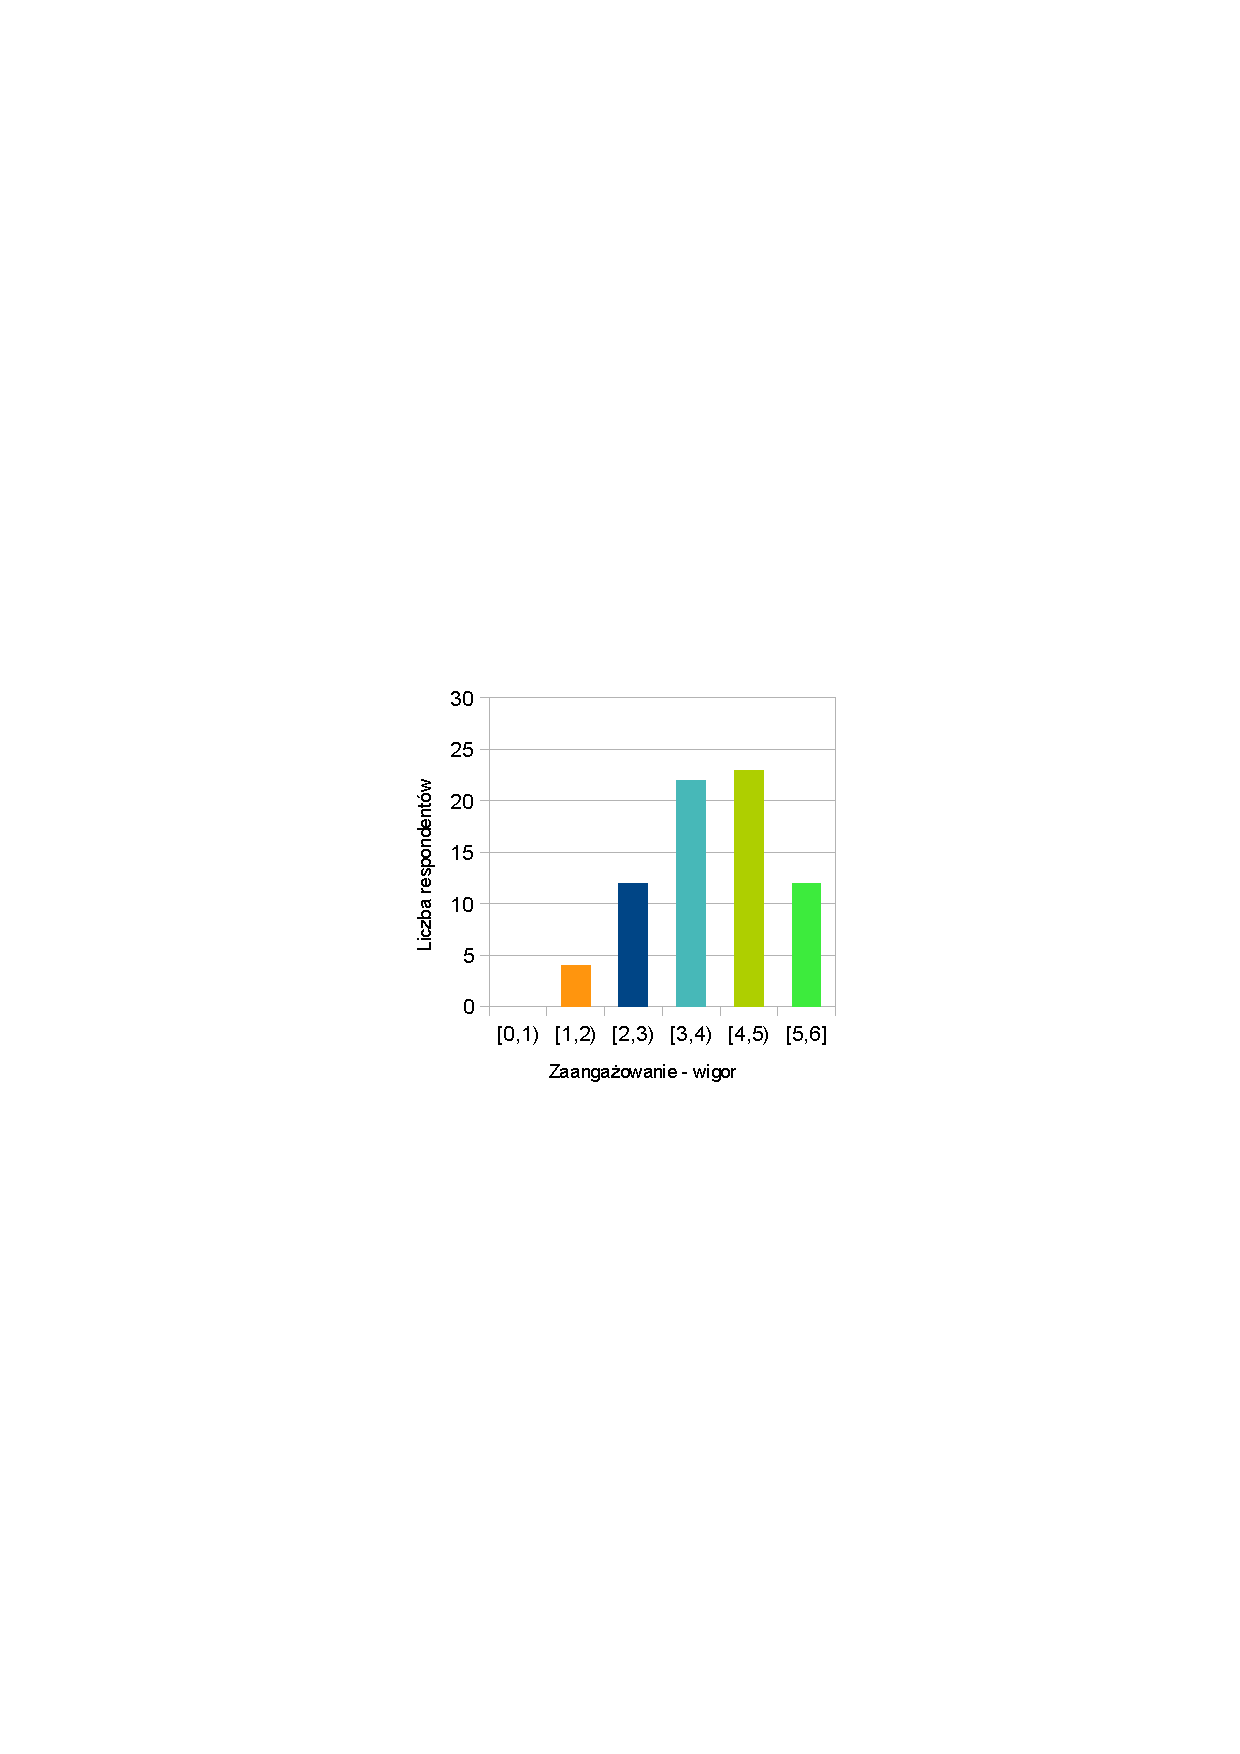
\includegraphics[height=0.27\textheight]{eng-vigor}}
    \subfloat[Oddanie]{\label{fig:eng-dedication}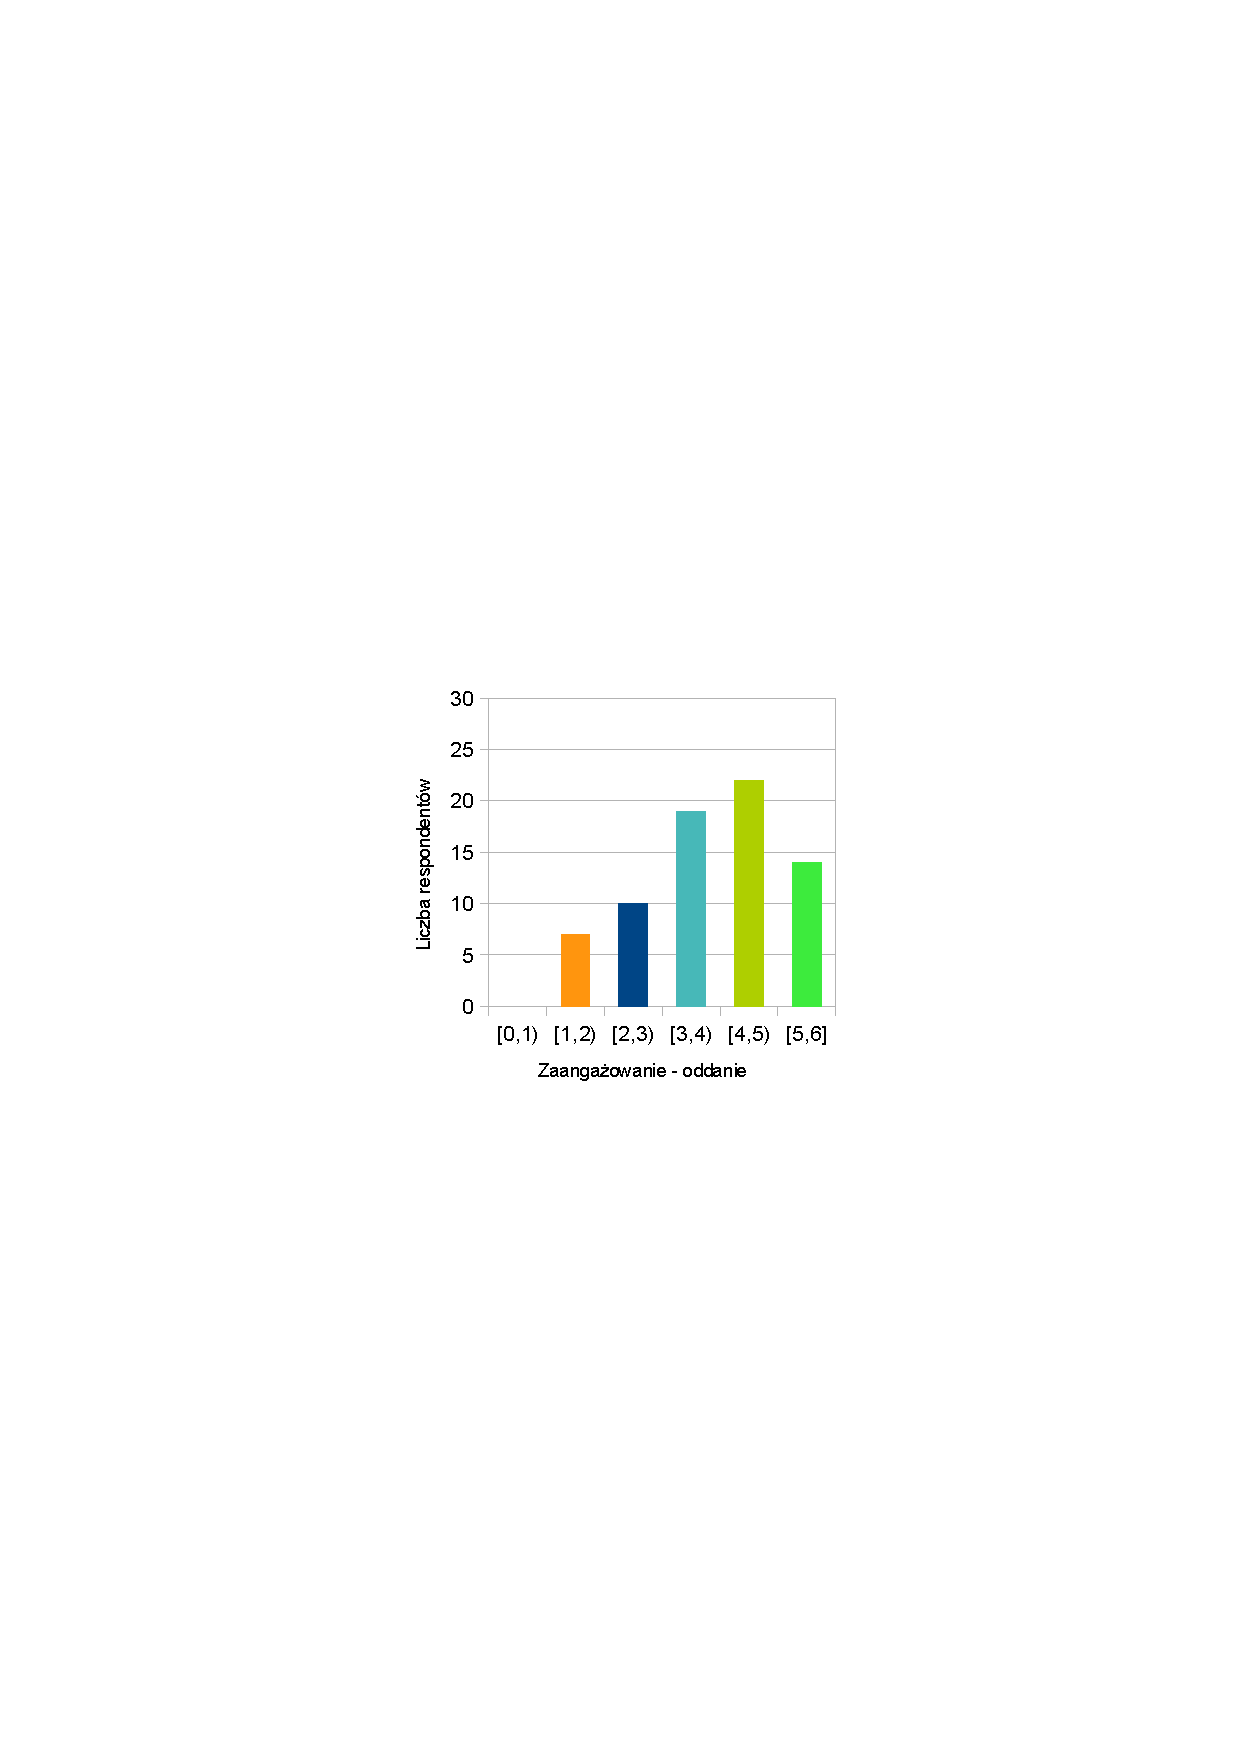
\includegraphics[height=0.27\textheight]{eng-dedication}}
    \\
    \subfloat[Absorpcja]{\label{fig:eng-absorption}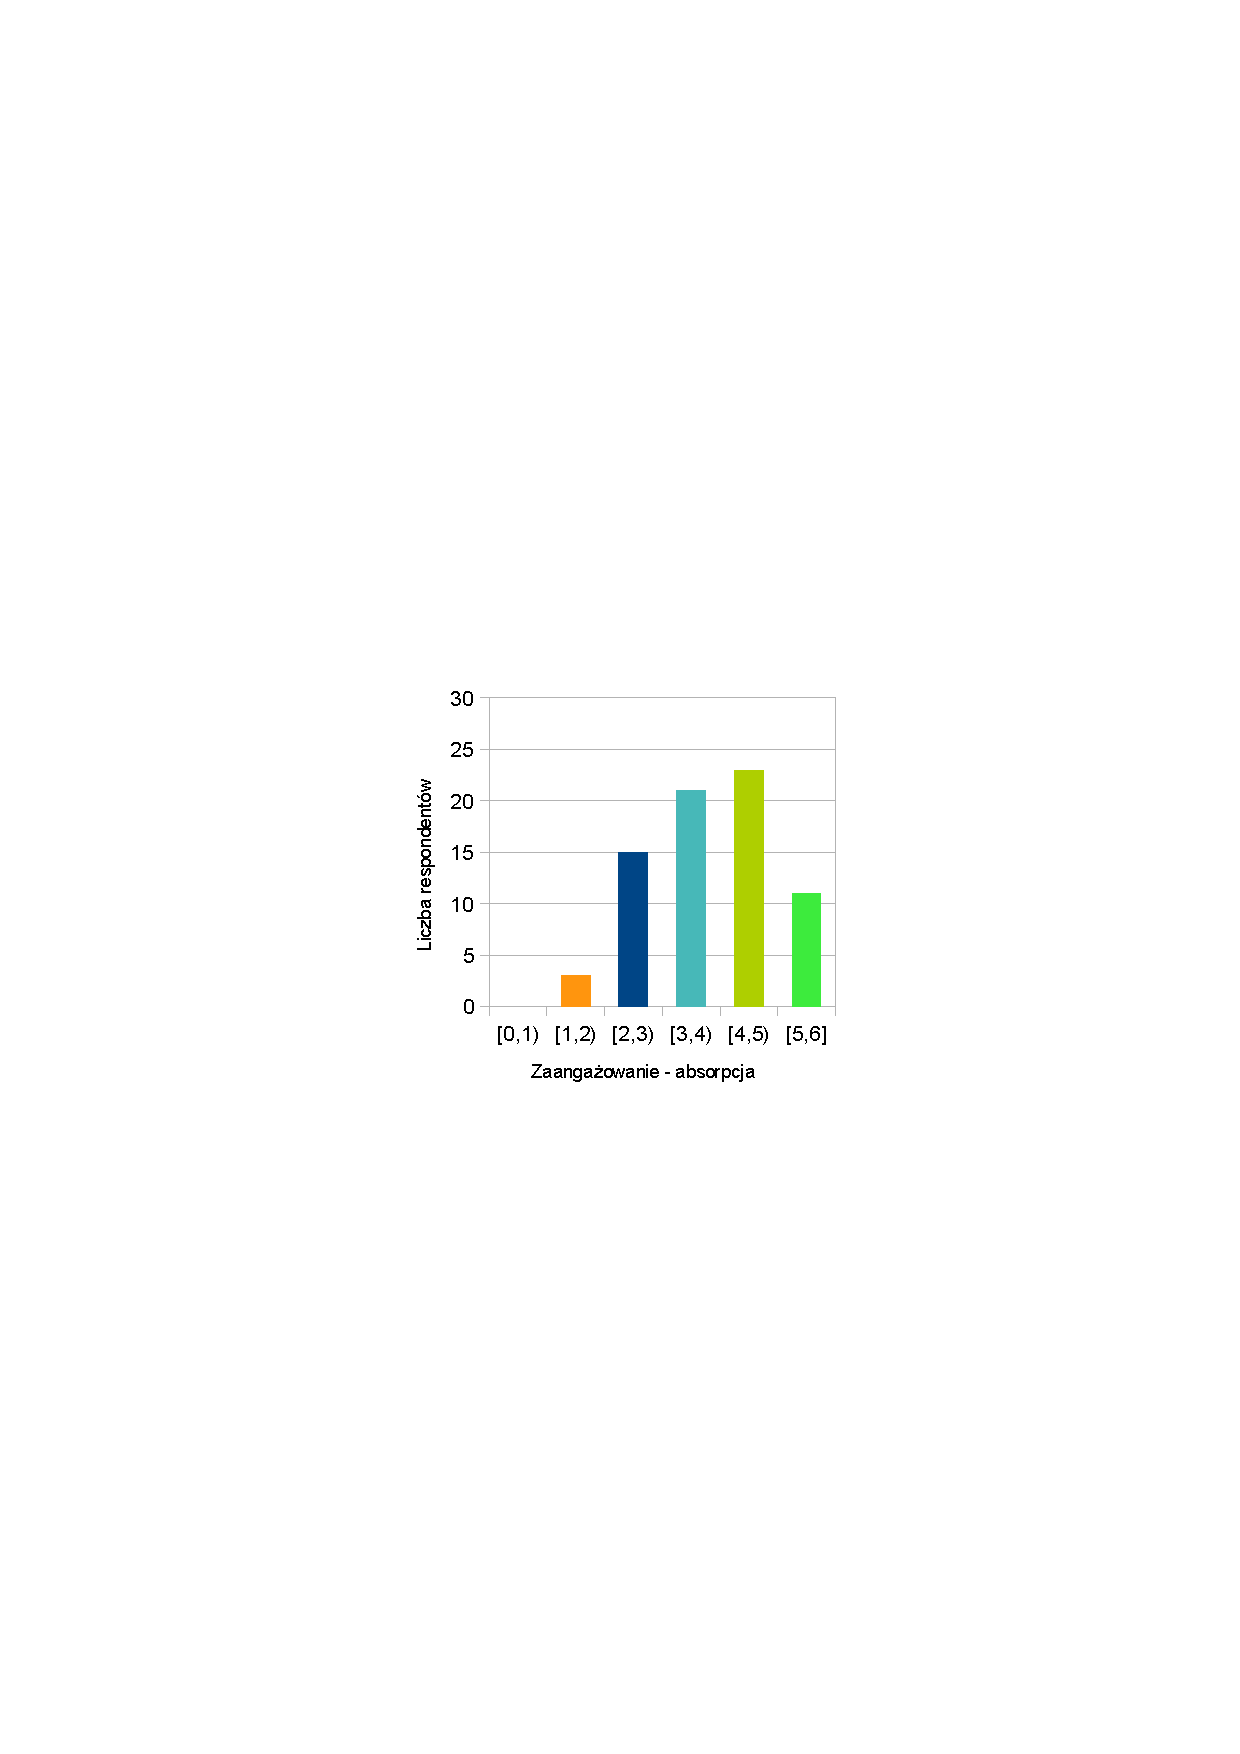
\includegraphics[height=0.27\textheight]{eng-absorption}}
    \subfloat[Zaangażowanie]{\label{fig:eng}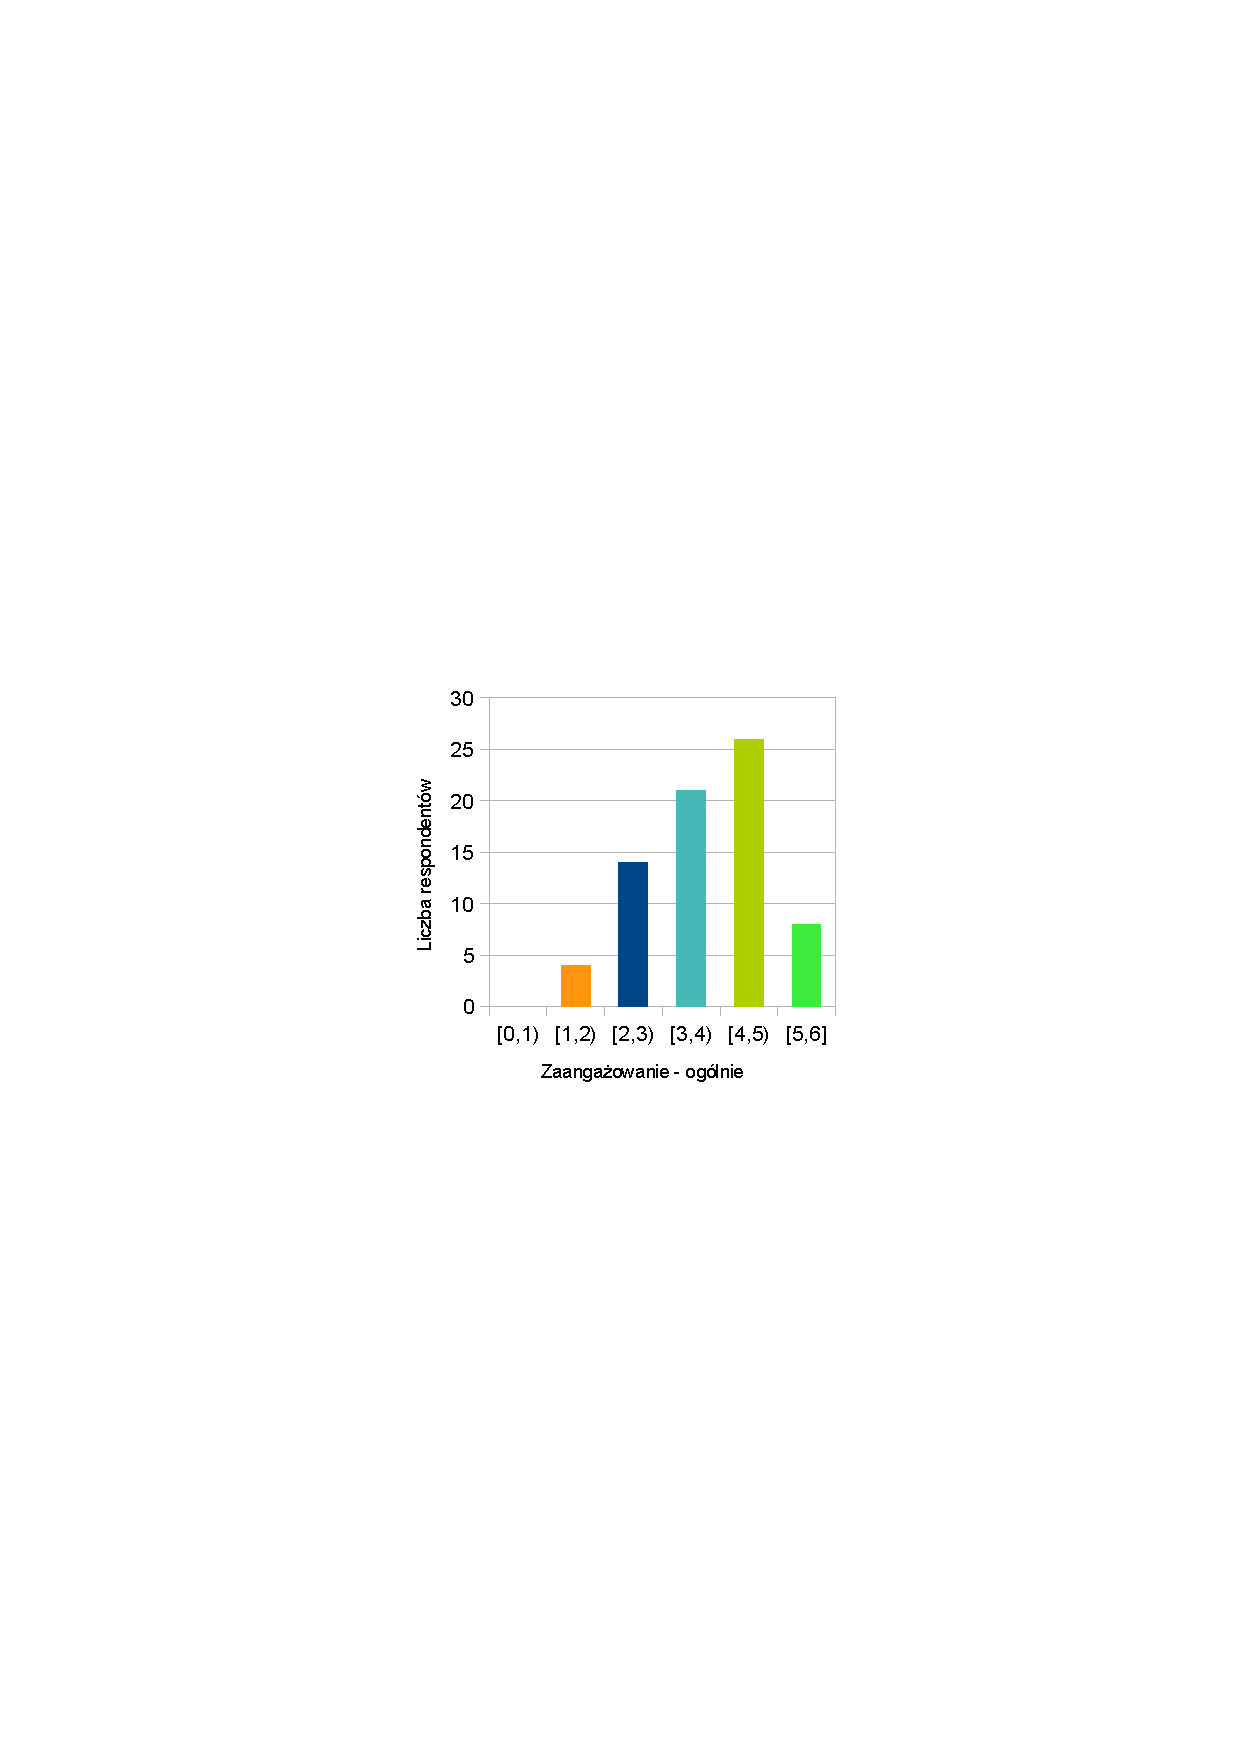
\includegraphics[height=0.27\textheight]{eng}}
    \caption{Histogramy dla \emph{UWES}}
\end{figure}

\begin{table}[h!]
\begin{center}
\begin{tabular}{l | c c c }
 & Wigor & Oddanie & Absorpcja \\ \hline \hline
Wigor & --- & 0,75 & 0,79 \\
Oddanie & & --- & 0,69 \\
Absorpcja & & & --- \\
\end{tabular}
\end{center}
\label{tab:uwes-correl}
\caption{Korelacja dla wszystkich wymiarów \emph{UWES}}
\end{table}

\paragraph{Wigor.} 

\paragraph{Oddanie.}

\paragraph{Absorpcja.}

\paragraph{Zaangażowanie ogólne.}


\section{Weryfikacja problemów badawczych}
\label{sec:hyp-ver}
\subsection{Zależność między satysfakcją, a zaangażowaniem}
\paragraph{Badanie}
Do badania zależności między satysfakcją, a zaangażowaniem wykorzystano współczynnik korelacji (przy istotności statystycznej 0,05). Obliczenia dla każdej z par wymiarów, jak i sumarycznych wyników znajdują się w Tabeli \ref{tab:jss-uwes-correl}.

\begin{table}[h!]
\begin{center}
\begin{tabular}{l || c c c | c}
  & Wigor & Oddanie & Absorpcja & Zaangażowanie \\ \hline \hline
Płaca & 0,18 & 0,32 & 0,24 & 0,27 \\
Awanse & 0,23 & 0,34 & 0,16 & 0,26 \\
Nadzór & 0,17 & 0,37 & 0,21 & 0,27 \\
Dodatki & 0,19 & 0,19 & 0,08 & 0,17 \\
Nagrody & 0,27 & 0,3 & 0,24 & 0,29 \\
\textcolor{Mahogany}{Organizacja pracy} & \textcolor{Mahogany}{-0,04} & \textcolor{Mahogany}{-0,1} & \textcolor{Mahogany}{-0,03} & \textcolor{Mahogany}{-0,06} \\
Współpracownicy & 0,32 & 0,39 & 0,22 & 0,34 \\
\textcolor{OliveGreen}{Wykonywana praca} & \textcolor{OliveGreen}{0,62} & \textcolor{OliveGreen}{0,79} & \textcolor{OliveGreen}{0,53} & \textcolor{OliveGreen}{0,71} \\
Komunikacja & 0,31& 0,38 & 0,33 & 0,38 \\ \hline
Satysfakcja & 0,36 & 0,48 & 0,32 & 0,42 \\ \hline
\end{tabular}
\end{center}
\caption{Korelacja między zaangażowaniem w pracę, a satysfakcję z pracy wraz z ich wymiarami.}
\label{tab:jss-uwes-correl}
\end{table}

\FloatBarrier

\paragraph{Dyskusja}
Jak widać w Tabeli \ref{tab:jss-uwes-correl}, między satysfakcją z pracy, a zaangażowaniem w pracę jest tylko średniej mocy zależność (wartość 0,42). Częściowo potwierdza to hipotezę postawioną w rozdziale \ref{sec:hypothesis-relation} ponieważ nie jesteśmy w stanie odrzucić istnienia zależności, ale też z całą pewnością jej potwierdzić. Wydawać by się mogło, że zgodnie z teorią satysfakcji \cite{SchultzSat} opisaną w rozdziale \ref{sec:theory-sat}:

\begin{quote}
  Zależy ona [\textit{satysfakcja z pracy}] od wielu czynników związanych z pracą (\ldots) do poczucia samospełnienia przy realizacji codziennych zadań.
\end{quote}

istnieje powiązanie z zaangażowaniem w pracę. W końcu fragment ten wydaje się być zbieżny z teorią Kahna odnoszącą się do wyrażania siebie w pracy (patrz rozdział \ref{sec:theory-eng-kahn}). W szczególności przytoczony cytat przypomina o wymiarach \textit{absorpcji} i \textit{wigoru}. 

Co ciekawe nie ma kompletnie relacji między wymiarem satysfakcji -- \textit{organizacja pracy}, a \textit{zaangażowaniem}. Podobna sytuacja jest ze \textit{współpracownikami} czy \textit{nadzorem}. Jest to niezgodne z teorią opisaną w rozdziałach o wpływie zaangażowania na pracownika i vice versa (rozdział \ref{sec:theory-eng-infl} -- ,,Zasoby w pracy'', rozdział \ref{sec:thoery-eng-infl2} -- ,,Pozytywne zachowania''). Z Tabeli \ref{tab:jss-uwes-correl} wynika, że warunki w pracy kompletnie nie mają wpływu na poziom naszej energii, stopień skupienia na zadaniu czy na oddanie
wykonywanej pracy. Pomimo tego, że to właśnie odpowiednie warunki i środowisko pracy powinno sprzyjać choćby wymiarowi \textit{absorpcja}. Jednak zależność między \textit{absorpcją}, a \textit{zaangażowaniem} wynosi
-0,03, zdecydowany brak jakiejkolwiek relacji przyczynowo-skutkowej. Wszystkie odpowiedzi badanych bazują na ich percepcji i ocenie różnych aspektów pracy. Respondenci mogą być nieświadomi braków, na którymkolwiek z wymiarów, które później mogą wpływać na inne aspekty czy emocje związane z pracą. W związku z tym warto zadać pytanie: czy niska wartość korelacji między \textit{organizacja pracy}, a \textit{zaangażowaniem} wskazuje, że badani nie są świadomi jak ten aspekt pracy wpływa na ich \textit{absorpcję} podczas pracy? Idąc dalej, jakie mają oczekiwania wobec
\textit{organizacji pracy}?

Z drugiej strony okazało się, że istnieje zależność między aspektem satysfakcji --\textit{wykonywana praca}, a \textit{zaangażowaniem} (wartość 0,71). Korelacje dla wspomnianego wymiaru satysfakcji oraz każdego z poszczególnych wymiarów zaangażowania są także wysokie:
\begin{itemize}
  \item cor(\textit{wykonywana praca}, \textit{oddanie}) = 0,79
  \item cor(\textit{wykonywana praca}, \textit{wigor}) = 0,62
  \item cor(\textit{wykonywana praca}, \textit{absorpcja}) = 0,53
\end{itemize}
Jak widać rodzaj wykonywanych zadań ma największy wpływ na oddanie pracy, czyli na uczucie dumy z wykonywanej pracy oraz jej sensowność w oczach pracownika. Oznacza to, że jeżeli ludzie lubią i cenią to co robią, sprzyja to ich oddaniu. 

Następny w kolejności wynik ma \textit{wigor}. Wydaje się być naturalnym, że skoro jesteśmy zadowoleni z wykonywanej pracy łatwiej nam włożyć w nią więcej energii, mamy więcej motywacji i siły do pokonywania przeszkód, które się pojawią w trakcie
realizacji zadań (i vice versa). 

Ostatnim wymiarem, ze średniej mocy zależnością, jest \textit{absorpcja}. Skoro lubimy wykonywać naszą pracą, nie wydaje się dziwnym to, że czas podczas jej wykonywania czas płynie bardzo szybko i potrafimy się całkowicie na niej skupić. 

Należy jednak postawić pytanie: dlaczego \textit{absorpcja} ma tylko średniej mocy relację z \textit{wykonywaną pracą}? Dlaczego kolejność siły zależności wygląda w ten sposób? Prawdopodobnie ma to związek z formą postawionych pytań w kwestionariuszu \emph{JSS}. Połowa pytań dla wymiaru \textit{wykonywana praca} (patrz dodatek \ref{sec:jss-text}) to:
\begin{quote}
  Czasami myślę, że moja praca jest bez sensu.
\end{quote}
\begin{quote}
  Jestem dumny z mojej pracy.
\end{quote}
Wydają się one odzwierciedlać idealnie \textit{oddanie}, czyli wymiar z najsilniejszą korelacją. Kolejne dwa pytania odnoszą się do lubienia pracy i odczuwania przyjemności podczas wykonywania zadań, które faktycznie mogą mieć związek z \textit{wigorem} i \textit{absorpcją}.


\subsection{Satysfakcja z pracy wśród sektora IT, a polskie normy}
\paragraph{Badanie}
\begin{hyp}
  Pracownicy sektora IT są bardziej zadowoleni z pracy niż przeciętni Polacy.
  \label{hip:sat}
\end{hyp}

W celu zweryfikowania Hipotezy \ref{hip:sat} przeprowadzono test różnic dla dwóch zmiennych niezależnych przy pomocy statystyki Z:

\begin{equation}
  Z = \frac{\overline{X_2} - \overline{X_1}}{\sqrt{\frac{\sigma^2_2}{N_2}+\frac{\sigma^2_1}{N_1}}}
\end{equation}

Dla badań populacji estymatory ($\overline{X}$) to średnie ($\mu$) dla badanych cech. Czyli badaną hipotezę statystyczną można przedstawić w następujący sposób:

\begin{equation}
  H0: \mu_{PL} = \mu_{IT} \qquad H1: \mu_{PL} < \mu_{IT}
\end{equation}

\begin{table}[h!b]
  \begin{center}
    \begin{tabular}{l | c c c }
      Satysfakcja & N & Śr. & War. \\ \hline
      sektor IT & 73 & 4,16 & 0,50 \\
      Polacy & 521 & 3,70 & 0,38 \\
    \end{tabular}
  \end{center}
  \caption{Statystyki opisowe potrzebne do wyliczenia statystyki Z.}
  \label{tab:jss-norms-data}
\end{table}

Do obliczenia statystyki Z wykorzystano dane z Tabeli \ref{tab:jss-norms-data}. Przy czym wybrano próg istotności statystycznej $\alpha = 0,05$, czyli $Z_{kryt.} = -1,64$.

\begin{equation}
  Z = \frac{\overline{X_{PL}} - \overline{X_{IT}}}{\sqrt{\frac{\sigma^2_{PL}}{N_{PL}}+\frac{\sigma^2_{IT}}{N_{IT}}}} = \frac{\mu_{PL} - \mu_{IT}}{\sqrt{\frac{\sigma^2_{PL}}{N_{PL}}+\frac{\sigma^2_{IT}}{N_{IT}}}} = \frac{3,70 - 4,16}{\sqrt{\frac{0,38}{521}+\frac{0,50}{73}}} = -5,29 
\end{equation}

Na podstawie niespełniania zależności:

\begin{equation}
  Z_{kryt.} < Z
\end{equation}

można odrzucić $H0: \mu_{PL} = \mu_{IT}$ oraz przyjąć $H1: \mu_{PL} < \mu_{IT}$ przy istotności statystycznej na poziomie $\alpha = 0,05$.

\paragraph{Dyskusja}
Jak widać z powyższych badań pracownicy sektora IT są bardziej zadowoleni z pracy niż przeciętni Polacy. 

Nasza grupa badanych jest dosyć młoda (patrz rozdział \ref{sec:group-age}), czyli teoretycznie ich zadowolenie powinno być niższe (zgodnie z rozdziałem \ref{sec:theory-sat} -- ,,Wpływ cech indywidualnych pracownika``). Warto tutaj przypomnieć fragment definicji satysfakcji z pracy z rozdziału \ref{sec:theory-sat} \cite{SchultzSat}:
\begin{quote}
  Nasza motywacja i aspiracje, oraz sposób ich zaspokajania przez pracę, także wpływają na postawy wobec pracy. [w tym satysfakcję z pracy]
\end{quote}
Widzimy, że sektor IT ma bardzo dużo do zaoferowania osobom z krótkim doświadczeniem zawodowym (patrz rozdział \ref{sec:group-exp}). Nawet w porównaniu z ogółem Polaków (przekrój lat doświadczenia o wiele szerszy), wypadają lepiej jeżeli chodzi o poziom satysfakcji z pracy.

Wynik ten jest także ciekawy kiedy weźmiemy pod uwagę teorię wpływu Locke'a (rozdział \ref{sec:theory-sat-locke}) o dopasowaniu oczekiwań, a zastaną sytuacją w pracy, jako główny czynnik wpływający na satysfakcję z pracy. Studia informatyczne są bardzo praktycznymi studiami. Dzięki przystępnym cenom sprzętu komputerowego oraz udostępnianiu dużej części narzędzi za darmo w Internecie (ruch
\href{http://en.wikipedia.org/wiki/Open-source_software}{OpenSource} oraz \href{http://en.wikipedia.org/wiki/Free_software}{FreeSoftware}) w bardzo łatwy sposób można odtworzyć środowisko pracy w laboratorium na uczelni, jak i w domu. Dzięki projektom zaliczeniowym w grupach studenci uczą się pracować w zespołach, jak to ma miejsce w środowisku pracy. Możliwe, że dzięki takiemu procesowi nauczania, który jest zbieżny z rzeczywistością zastaną w pracy, oczekiwania ludzi
wkraczających na rynek pracy nie odbiegają zbytnio od zastanych. Stąd może wynikać większa satysfakcja z pracy wśród pracowników sektora IT niż normy dla wszystkich Polaków. W końcu normy tworzony są na podstawie uśredniania po wszystkich grupach zawodowych (grupa ogółu Polaków).

Natomiast patrząc na obecne wyniki z punktu widzenia teorii Herzberga (rozdział \ref{sec:theory-sat-herz}) wszystkie czynniki higieny jakie badaliśmy są spełnione (większość respondentów jest usatysfakcjonowana z odpowiadających wymiarów pracy). Ponadto z badanych motywatorów, z jednego są usatysfakcjonowani (docenienie, patrz wymiar \textit{nagrody} w teście \emph{JSS}), z jednego mają mieszane uczucia (możliwości promocji, patrz wymiar \textit{awans} w teście \emph{JSS}). Z czego można wywnioskować, że
grupa respondentów powinna być raczej zadowolona ze swojej pracy, skoro brak jest czynników powodujących zmniejszenie satysfakcji (niezadowolenie na czynnikach higieny) oraz istnieją czynniki powodujące ich wzrost (zadowolenie na chociaż jednym motywatorze). 

Poniżej znajduje się lista motywatorów i czynników higieny badanych przez \emph{JSS} oraz wyniki jakie zostały uzyskane podczas badania.

\begin{itemize}
  \item motywator \textit{docenienie} $\rightarrow$ wymiar \textit{nagrody} (śr. 15,86),
  \item motywator \textit{możliwości promocji} $\rightarrow$ wymiar \textit{awanse} (śr. 13,47),
  \item czynnik higieny \textit{płaca} $\rightarrow$ wymiar \textit{płaca} (śr. 15,99),
  \item czynnik higieny \textit{nadzór} $\rightarrow$ wymiar \textit{nadzór} (śr. 19.18),
  \item czynnik higieny \textit{organizacja w firmie} $\rightarrow$ wymiar \textit{warunki} (śr. 15,51).
\end{itemize}

Co ciekawe, pomimo tego że mamy młodą grupę badanych, są oni usatysfakcjonowani swoją pracę. Jest to sprzeczne z opisem wypływu wieku na zadowolenie z pracy z rozdziału \ref{sec:theory-sat-age}. Jednak jeżeli zwrócimy uwagę na wymiar \textit{awansów}, gdzie tyle samo osób jest zadowolonych i tyle samo niezadowolonych, oraz spojrzymy na doświadczenie naszej grupy (co najwyżej kilkuletnie) i zajmowane stanowiska (głównie specjaliści różnego stopnia), widzimy, że pomimo młodego wieku
osoby te mają szanse na awans oraz pracują na znaczących pozycjach (większość to specjaliści).

Za to zgodnie z opisem zależności dla zdolności poznawczych w rozdziale \ref{sec:theory-sat-age}, osoby badane są głównie zadowolone ze swojej pracy. Należy tutaj pamiętać, że większość osób pracuje jako specjaliście różnego szczebla, więc ich zdolności poznawcze powinny być wysokie.

Potwierdzają się także badania odnośnie zachowań prospołecznych (patrz rozdział \ref{sec:theory-sat-infl} -- ,,Zachowania prospołeczne i nieproduktywne``). Większość osób jest zadowolonych ze swojej pracy i jednocześnie bardzo wysoko ocenia swoich współpracowników (wymiar \textit{współpracownicy}).
\subsection{Zaangażowanie w pracę wśród sektora IT, a polskie normy}
\paragraph{Badanie}
\begin{hyp}
  Pracownicy sektora IT są bardziej zaangażowani w pracę niż przeciętni Polacy.
  \label{hip:eng}
\end{hyp}

Podobnie jak w przypadku satysfakcji, aby zbadać prawdziwość Hipotezy \ref{hip:eng} przeprowadzono test różnic dla dwóch zmiennych niezależnych przy pomocy statystyki Z:

\begin{equation}
  Z = \frac{\overline{X_2} - \overline{X_1}}{\sqrt{\frac{\sigma^2_2}{N_2}+\frac{\sigma^2_1}{N_1}}}
\end{equation}

Badana hipoteza statystyczna  to:

\begin{equation}
  H0: \mu_{PL} = \mu_{IT} \qquad H1: \mu_{PL} < \mu_{IT}
\end{equation}

\begin{table}[h!b]
  \begin{center}
    \begin{tabular}{l | c c c }
      Zaangażowanie & N & Śr. & War. \\ \hline
      sektor IT & 73 & 3,76 & 1,04 \\
      Polacy & 1438 & 3,86 & 0,90 \\
    \end{tabular}
  \end{center}
  \caption{Statystyki opisowe potrzebne do wyliczenia statystyki Z.}
  \label{tab:uwes-norms-data}
\end{table}

Do obliczenia statystyki Z wykorzystano dane z Tabeli \ref{tab:uwes-norms-data} przy progu istotności statystycznej $\alpha = 0,05$, czyli $Z_{kryt.} = -1,64$.

\begin{equation}
  Z = \frac{\overline{X_{PL}} - \overline{X_{IT}}}{\sqrt{\frac{\sigma^2_{PL}}{N_{PL}}+\frac{\sigma^2_{IT}}{N_{IT}}}} = \frac{\mu_{PL} - \mu_{IT}}{\sqrt{\frac{\sigma^2_{PL}}{N_{PL}}+\frac{\sigma^2_{IT}}{N_{IT}}}} = \frac{3,86- 3,76}{\sqrt{\frac{0,90}{1438}+\frac{1,04}{73}}} = 0,19
\end{equation}

Na podstawie spełnienia zależności:

\begin{equation}
  Z_{kryt.} < Z
\end{equation}

można przyjąć $H0: \mu_{PL} = \mu_{IT}$ oraz odrzucić $H1: \mu_{PL} < \mu_{IT}$ przy istotności statystycznej na poziomie $\alpha = 0,05$.

\paragraph{Dyskusja}
Jak widać z powyższego testu statystycznego, pracownicy sektora IT są tak samo zaangażowani w pracę jak przeciętni Polacy.

Wyrażając wynik przy pomocy definicji Kahna (patrz rozdział \ref{sec:theory-eng-kahn}), informatycy nie wyrażają siebie w pracy lepiej niż przeciętni Polacy. Pytanie, czy istnieje powód, aby było na odwrót? W obecnych czasach sami decydujemy o wyborze zawodu, a co za tym idzie jak będziemy wyrażać się pracy. Jak widać, statystycznie rzecz biorąc, pracownicy sektora IT nie różnią się tutaj od przeciętnego Polaka. Wynika z tego, że podobny odsetek osób jest dopsaowanych do
wykonywanego zawodu (tzw. odpowiedniość pracy).

Z kolei z perspektywy teorii Maslacha, Jacksona i Leitera (patrz rozdział \ref{sec:model-maslach}) badana grupa nie jest bardziej wypalona w pracy niż ogół. Mają podobną energię w pracy, stosunek do niej (cynizm lub entuzjazm) oraz wykazują taką samą skuteczność podczas wykonywania zadań. Czyli badana grupa nie posiada żadnych specyficznych cech, które wyróżniałyby ich na tle ogółu Pokaów i predysponowały do zwiększonego zaangażowania w pracę. Co ciekawe grupa badanych
jest młoda oraz większość osób pracuje na stanowiskach specjalistycznych (pomimo wieku). Jednak nie wpływa to w żaden sposób na
ilość osób zaangażowanych czy wypalonych osób. Wydawać by się mogło, że młode osoby powinny później ulegać wypaleniu zawodowemu. Jednak nie ma to odzwierciedlenia w niniejszych badaniach.

Patrząc na ostatnią teorię Schaufelliego oraz Bakkera (patrz rozdział \ref{sec:model-schauffeli}) możemy powiedzieć, że respondenci z podobną częstotliwością oraz w podobny sposób odczuwają pozytywne uczucia spełnienia związane z wykonywaną pracą, a w szczególności \textit{wigor}, \textit{oddanie} i \textit{absorpcję}. Co ciekawe nie ma to nic wspólnego z odpowiedniością pracy (patrz wysokie wyniki z satysfakcji na wymiarze \textit{wykonywana praca}). Tym bardziej
jeżeli chodzi o ostatni wymieniony wymiar zaangażowania związany z wgłębieniem się w zadania oraz skupieniu nad pracą. Wydaje się to być zaskakujące.


\cleardoublepage
\appendix
\section{Polskie tłumaczenia}

\subsection{\emph{Job Satisfaction Survey}}
\label{sec:jss-text}
\paragraph{Płaca}
\begin{enumerate}
  \item Uważam, że płacą mi odpowiednio za pracę którą wykonuję.
  \item Podwyżki zdarzają się zbyt rzadko.
  \item Gdy myślę o swoim wynagrodzeniu, czuję się niedoceniany.
  \item Jestem usatysfakcjonowany perspektywą wzrostu zarobków w przyszłości.
\end{enumerate}

\paragraph{Awans}
\begin{enumerate}
  \item W mojej firmie są małe szanse na awans w pracy.
  \item Ten kto dobrze wykonuje swoją pracę ma u nas spore szanse na awans.
  \item Ludzie awansują w mojej firmie tak szybko jak w innych firmach.
  \item Jestem zadowolony z możliwości awansu.
\end{enumerate}

\paragraph{Nadzór}
\begin{enumerate}
  \item Mój kierownik jest całkiem kompetentny w wykonywaniu swojej pracy.
  \item Mój kierownik jest wobec mnie niesprawiedliwy.
  \item Mój kierownik za mało interesuje się odczuciami podwładnych.
  \item Lubię mojego kierownika.
\end{enumerate}

\paragraph{Świadczenia pracownicze}
\begin{enumerate}
  \item Nie jestem zadowolony ze świadczeń, które otrzymuje.
  \item Świadczenia, które otrzymuję są porównywalne z tymi, które oferuje większość innych firm.
  \item Pakiet świadczeń, który otrzymuje, jest słuszny.
  \item Są dodatkowe świadczenia, których nie otrzymuję, a uważam, że powinienem.
\end{enumerate}

\paragraph{Warunkowe nagrody}
\begin{enumerate}
  \item Gdy dobrze wykonuje pracę jestem odpowiednio doceniany.
  \item Uważam, że moja praca jest niedoceniana.
  \item Jest mało nagród dla tych, którzy tu pracują.
  \item Uważam, że moje wysiłki nie są nagradzane w sposób w jaki być powinny.
\end{enumerate}

\paragraph{Organizacja pracy}
\begin{enumerate}
  \item Wiele naszych reguł i procedur utrudnia dobre wykonywanie pracy.
  \item Biurokracja rzadko przeszkadza mi dobrze wykonywać swoją pracę.
  \item Mam za dużo zadań do wykonania w pracy.
  \item Mam za dużo papierkowej roboty.
\end{enumerate}

\paragraph{Współpracownicy}
\begin{enumerate}
  \item Lubię ludzi, z którymi pracuję.
  \item Uważam, że muszę pracować ciężej z powodu niekompetencji osób, z którymi pracuję.
  \item Lubię spędzać czas ze swoimi współpracownikami.
  \item W pracy jest za dużo sprzeczek oraz konfliktów wewnętrznych.
\end{enumerate}

\paragraph{Wykonywana praca}
\begin{enumerate}
  \item Czasami myślę, że moja praca jest bez sensu.
  \item Lubię rzeczy, którymi się zajmuje w mojej pracy.
  \item Jestem dumny z mojej pracy.
  \item Moja praca jest przyjemna.
\end{enumerate}

\paragraph{Komunikacja}
\begin{enumerate}
  \item Komunikacja w mojej firmie wydaje się dobra.
  \item Cele firmy, dla której pracuje, są dla mnie niejasne.
  \item Często mam odczucie, że nie wiem co się dzieje w mojej firmie.
  \item Przydzielane zadania nie są w pełni wyjaśniane.
\end{enumerate}

\subsection{\emph{Utrecht Work Engagement Survey}}
\label{sec:uwes-text}
\paragraph{Wigor}
\begin{enumerate}
  \item W pracy czuję, że rozpiera mnie energia.
  \item W pracy czuję się silny i pełny energii.
  \item Kiedy rano wstaję, mam ochotę iść do pracy.
  \item Mogę kontynuować pracę przez bardzo długie odcinki czasu.
  \item W pracy jestem odporny psychicznie.
  \item Zawsze pracuję wytrwale, nawet gdy sprawy nie idą dobrze.
\end{enumerate}

\paragraph{Oddanie}
\begin{enumerate}
  \item Praca, którą wykonuję, jest dla mnie pełna sensu i celowości.
  \item Jestem pełen entuzjazmu w stosunku do swojej pracy.
  \item Moja praca jest dla mnie natchnieniem.
  \item Jestem dumny z pracy, którą wykonuje.
  \item Praca jest dla mnie pełna wyzwań.
\end{enumerate}

\paragraph{Absorpcja}
\begin{enumerate}
  \item Czas mi szybko leci kiedy pracuje.
  \item Kiedy pracuję, zapominam o wszystkim dookoła mnie.
  \item Czuję się szczęśliwy kiedy intensywnie pracuję.
  \item Jestem pochłonięty swoją pracą.
  \item Zdarza się, że się zapominam w pracy.
  \item Trudno mi się oderwać od mojej pracy.
\end{enumerate}
\cleardoublepage
\section{Polskie normy}
\subsection{Satysfakcja z pracy}
\label{sec:app-jss-norms}

\begin{table}[h!]
\begin{center}
\begin{tabular}{l | c c c c c}
  & Liczba & Min. & Max. & Śr. & Od. std. \\ \hline
Płaca & 521 & 1,00 & 6,00 & 3,2367 & 1,19249 \\
Awanse & 521 & 1,00 & 6,00 & 3,0893 & 1,15440 \\ 
Nadzór &  521 & 1,00 & 6,00 & 3,9715 & 1,16198 \\
Dodatki &  521 & 1,00 & 6,00 & 3,5974 & 1,00897 \\
Nagrody &  521 & 1,00 & 6,00 & 3,5717 & 0,78612 \\
Warunki &  521 & 1,00 & 6,00 & 3,6243 & 1,02717 \\
Współpracownicy &  521 & 1,00 & 6,00 & 4,1961 & 1,04071 \\
Wykonywana praca &  521 & 1,00 & 6,00 & 4,2035 & 1,15145 \\
Komunikacja & 521 & 1,00 & 6,00 & 3,9301 & 1,04113 \\ \hline
Satysfakcja & 521 & 1,29 & 5,74 & 3,6967 & 0,61543 \\
\end{tabular}
\end{center}
\caption{Polskie normy dla satysfakcji z pracy.}
\label{tab:jss-pl-norms}
\end{table}

\FloatBarrier

\subsection{Zaangażowanie w pracę}
\label{sec:app-uwes-norms}

\begin{table}[h!]
\begin{center}
\begin{tabular}{l | c c c c c}
  & Liczba & Min. & Max. & Śr. & Od. std. \\ \hline
Wigor & 1438 & 0,00 & 6,00 & 3,9857 & 0,96209 \\
Oddanie & 1438 &  0,00 & 6,00 & 3,8424 & 1,24056 \\
Absorpcja & 1438 & 0,00 & 6,00 & 3,7408 & 1,01110 \\ \hline
Zaangażowanie & 1438 & 0,71 & 6,00 & 3,8572 & 0.95049 \\
\end{tabular}
\end{center}
\caption{Polskie normy dla zaangażowania w pracę.}
\label{tab:uwes-pl-norms}
\end{table}

\FloatBarrier

\end{document}
